\documentclass[a4paper]{article}
\usepackage{vntex}
%\usepackage[english,vietnam]{babel}
%\usepackage[utf8]{inputenc}
\usepackage{mathptmx}[ptm]
%\usepackage[utf8]{inputenc}
%\usepackage[francais]{babel}
\usepackage{a4wide,amssymb,epsfig,latexsym,array,hhline,fancyhdr}
\usepackage[normalem]{ulem}
%\usepackage{soul}

\usepackage[makeroom]{cancel}
\usepackage{amsmath}
\usepackage{amsthm}
\usepackage{multicol,longtable,amscd}
\usepackage{diagbox}%Make diagonal lines in tables
\usepackage{booktabs}
\usepackage{alltt}
\usepackage[framemethod=tikz]{mdframed}% For highlighting paragraph backgrounds
\usepackage{caption,subcaption}

\usepackage{lastpage}
\usepackage[lined,boxed,commentsnumbered]{algorithm2e}
\usepackage{enumerate}
\usepackage{color}
\usepackage{graphicx}							% Standard graphics package
\usepackage{array}
\usepackage{tabularx, caption}
\usepackage{multirow}
\usepackage{multicol}
\usepackage{rotating}
\usepackage{graphics}
\usepackage{geometry}
\usepackage{setspace}
\usepackage{epsfig}
\usepackage{tikz}
\usepackage{float}
\usetikzlibrary{arrows,snakes,backgrounds,calc}
\usepackage[unicode]{hyperref}
\hypersetup{urlcolor=blue,linkcolor=black,citecolor=black,colorlinks=true} 
\usepackage{listings}

%\usepackage{pstcol} 								% PSTricks with the standard color package

\usepackage[normalem]{ulem}

\newtheorem{theorem}{{\bf Định lý}}
\newtheorem{property}{{\bf Tính chất}}
\newtheorem{proposition}{{\bf Mệnh đề}}
\newtheorem{corollary}[proposition]{{\bf Hệ quả}}
\newtheorem{lemma}[proposition]{{\bf Bổ đề}}
\theoremstyle{definition}
\newtheorem{exer}{Bài toán}
\addtocontents{toc}{\protect\thispagestyle{empty}}
% Remove page number in contents page. 
\addtocontents{lof}{\protect\thispagestyle{empty}}
% Remove page number in list of figure page. 
\addtocontents{lot}{\protect\thispagestyle{empty}}
% Remove page number in list of table page. 
\def\thesislayout{	% A4: 210 × 297
	\geometry{
		a4paper,
		total={160mm,240mm},  % fix over page
		left=30mm,
		top=22mm,
            right=20mm,
            bottom=20mm,
	}
}
\def\thesisheadlayout{	% A4: 210 × 297
	\geometry{
		a4paper,
		total={160mm,240mm},  % fix over page
		left=30mm,
		top=10mm,
	}
}
\thesislayout
\lstset{
language=R,
basicstyle=\footnotesize\sffamily,
commentstyle=\ttfamily\color{black},
numbers=left,
numberstyle=\ttfamily\color{black}\footnotesize,
stepnumber=1,
numbersep=5pt,
backgroundcolor=\color{white},
showspaces=false,
showstringspaces=false,
showtabs=false,
frame=single,
tabsize=2,
captionpos=b,
breaklines=true,
breakatwhitespace=false,
title=\lstname,
escapeinside={},
keywordstyle={},
morekeywords={}
}
%\usepackage{fancyhdr}
\setlength{\headheight}{40pt}
\pagestyle{fancy}
\fancyhead{} % clear all header fields
\renewcommand{\footruleskip}{1mm}

\fancyhead[L]{
 \begin{tabular}{rl}
    \begin{picture}(25,15)(0,0)
    \put(0,-8){
\includegraphics[width=10mm, height=10mm]{Images/hcmut.png}}
    %\put(0,-8){\epsfig{width=10mm,figure=hcmut.eps}}
   \end{picture}&
	%
\includegraphics[width=8mm, height=8mm]{hcmut.png} & %
	\begin{tabular}{l}
		\textbf{  Trường Đại Học Bách Khoa - Đại học Quốc gia TP.HCM }\\
		\textbf{  Khoa Khoa Học \& Kỹ Thuật Máy Tính}
	\end{tabular} 	
 \end{tabular}
}
\fancyhead[R]{
	\begin{tabular}{l}
		\tiny \bf \\
		\tiny \bf 
	\end{tabular}  }
\fancyfoot{} % clear all footer fields
\fancyfoot[L]{\scriptsize  Báo cáo Đồ án chuyên ngành (CO4029) - HK1 2024 - 2025}
\fancyfoot[R]{\scriptsize  Trang {\thepage}/\pageref{LastPage}}

\renewcommand{\headrulewidth}{0.3pt}
\renewcommand{\footrulewidth}{0.3pt}

%%%
\setcounter{secnumdepth}{4}
\setcounter{tocdepth}{3}
\makeatletter
\newcounter {subsubsubsection}[subsubsection]
\renewcommand\thesubsubsubsection{\thesubsubsection .\@alph\c@subsubsubsection}
\newcommand\subsubsubsection{\@startsection{subsubsubsection}{4}{\z@}%
                                     {-3.25ex\@plus -1ex \@minus -.2ex}%
                                     {1.5ex \@plus .2ex}%
                                     {\normalfont\normalsize\bfseries}}
\newcommand*\l@subsubsubsection{\@dottedtocline{3}{10.0em}{4.1em}}
\newcommand*{\subsubsubsectionmark}[1]{}
\makeatother

\everymath{\color{black}}%make in-line maths symbols blue to read/check easily

\sloppy
\captionsetup[figure]{labelfont={small,bf},textfont={small,it},belowskip=-1pt,aboveskip=-9pt}
%space remove between caption, figure, and text
\captionsetup[table]{labelfont={small,bf},textfont={small,it},belowskip=-1pt,aboveskip=7pt}
\setlength{\floatsep}{5pt plus 2pt minus 2pt}
\setlength{\textfloatsep}{5pt plus 2pt minus 2pt}
\setlength{\intextsep}{10pt plus 2pt minus 2pt}

\thesislayout

\begin{document}

\begin{titlepage}
\begin{tikzpicture}[remember picture, overlay]
  \draw[line width = 4pt] ($(current page.north west) + (0.4in,-0.5in)$) rectangle ($(current page.south east) + (-0.4in,0.5in)$);
  \draw[line width=1.5pt]
    ($ (current page.north west) + (0.45in,-0.55in) $)
    rectangle
    ($ (current page.south east) + (-0.45in,0.55in) $);
\end{tikzpicture}

\begin{center}
\LARGE \textbf{ĐẠI HỌC QUỐC GIA THÀNH PHỐ HỒ CHÍ MINH} \\
\vspace{0.2cm}
\LARGE \textbf{TRƯỜNG ĐẠI HỌC BÁCH KHOA} \\
\vspace{0.2cm}
\LARGE \textbf{KHOA KHOA HỌC VÀ KĨ THUẬT MÁY TÍNH}
\end{center}

\vspace{0.3cm}

\begin{figure}[h!]
\begin{center}

\includegraphics[width=4cm]{Images/hcmut.png}
\end{center}
\end{figure}

\begin{center}
\begin{tabular}{c}
\multicolumn{1}{c}{\textbf{{\LARGE BÁO CÁO}}}\\
\\{\textbf{{\LARGE ĐỒ ÁN TỐT NGHIỆP}}}
% \\{\textbf{{\LARGE ĐỒ ÁN KỸ THUẬT MÁY TÍNH}}}
% \\{\textbf{{\LARGE ĐỒ ÁN MÔN HỌC}}}
% \\ \textit{(SV chọn tên môn học cho phù hợp)}
\\
\\
\textbf{\LARGE MEOWSQL KNIGHT - TRÒ CHƠI CHIẾN ĐẤU BẰNG SQL}
\\
\\
\\ \vspace{0.5cm} {\Large NGÀNH: KHOA HỌC MÁY TÍNH}
\end{tabular}
\end{center}
\vspace{0.5cm}


\begin{table}[h]
\begin{tabular}{rll}
\hspace{6 cm} &  \textbf{\Large HỘI ĐỒNG 2
	 KHOA HỌC MÁY TÍNH}
\\
\\
\hspace{6 cm} &   \textbf{\Large GVHD:} {\Large VƯƠNG BÁ THỊNH}
\\
\\
\hspace{6 cm}  &   \textbf{\Large GVPB:} {\Large TRẦN HUY}
\\
\\
% TKHĐ là THƯ KÝ HỘI ĐỒNG
\hspace{6 cm} &     \textbf{$\;$ $\;$$\;$$\;$$\;$$\;$$\;$$\;$$\;$$\;$$\;$$\;$$\;$$\;$$\;$$\;$$\;$$\;$$\;$$\;$$\;$$\;$$\;$$\;$$\;$$\;$$\;$$\;$$\;$$\;$$\;$$\;$$\;$$\;$ \Large ---o0o---} 
\\
\\
\hspace{6 cm} &   \textbf{\Large SVTH1:} {\Large Trần Đan Huy - 2111356}
\\
\\
\hspace{6 cm}&   \textbf{\Large SVTH2:}  {\Large Lê Quang Hiển - 2113376}
\\
\\

\end{tabular}
\end{table}

\vspace{0.5cm}
\begin{center}
{\Large TP. HỒ CHÍ MINH, 09/2025}
\end{center}
\end{titlepage}
%\thispagestyle{empty}
\newpage

%%%%%%%%%%%%%%%%%INTRO%%%%%%%%%%%%%%%%%%%
\section*{Lời cảm ơn}
\thispagestyle{empty}
\hspace*{0.5cm} Quá trình thực hiện đồ án là cả một quá trình của sự nỗ lực, trải qua nhiều cung bậc cảm xúc khác nhau, hỉ nộ ái ố đều có. Với sự nỗ lực không ngừng, không chịu bỏ cuộc của các thành viên trong nhóm cùng sự hỗ trợ không ngơi nghỉ của giảng viên hướng dẫn, nhóm đã có thể hoàn thiện đồ án chuyên ngành.\\
\hspace*{0.5cm} Nhóm xin bày tỏ lòng biết ơn vô cùng sâu sắc đến Thầy Vương Bá Thịnh, người đã tận tâm, tận lực hỗ trợ nhóm trong suốt quá trình thực hiện đồ án này. Những lời hướng dẫn, lời đánh giá và góp ý, cùng những đốc thúc, động viên của thầy đã góp một phần rất lớn trong việc giúp nhóm hoàn thiện đồ án trong giai đoạn thiết kế và đi vào giai đoạn hiện thực.\\
\hspace*{0.5cm} Ngoài ra, nhóm cũng xin cảm ơn các giảng viên tại Khoa Khoa học và Kỹ thuật Máy tính, Đại học Quốc gia TP. Hồ Chí Minh - Trường Đại học Bách Khoa vì những kiến thức vô cùng hữu ích mà các thầy, các cô đã tận tâm truyền đạt, những kiến thức này chính là nền tảng vô cùng quan trọng giúp các thành viên trong nhóm có thể thực hiện đồ án được tốt hơn và cũng tạo nên những cảm hứng cho nhóm áp dụng những kiến thức
đó vào dự án này và những dự án về sau.\\
\hspace*{1cm} Cuối cùng, nhóm xin gửi lời cảm ơn đến gia đình và bạn bè, những người luôn đồng hành và động viên nhóm trong suốt hành trình tại trường đại học. Đặc biệt là trong những giai đoạn khó khăn. Những lời nói ấy, cử chỉ động viên ấy đầy ắp sự yêu thương và đó là nguồn đồng lực giúp nhóm tiếp tục nỗ lực, vượt qua những khó khăn, thử thách, hướng tới chân trời mới, thành tựu mới.
 
\par\hfill\textbf{Nhóm tác giả}\hspace{1cm}
\par\hfill\textit{Trần Đan Huy}\hspace{1cm}
\par\hfill\textit{Lê Quang Hiển}\hspace{1cm}

\clearpage
\pagenumbering{arabic}

\section*{Lời cam đoan}
\thispagestyle{empty}

\hspace*{0.5cm} Nhóm xin cam đoan rằng mọi kết quả thu được trong quá trình thực hiện đồ án chuyên ngành này đều là kết quả của sự nỗ lực và làm việc chăm chỉ của bản thân. Tuyệt đối không có hành vi sao chép hoặc sử dụng công trình của người khác mà không trích dẫn đúng quy định. Trong trường hợp phát hiện bất kỳ hành vi vi phạm nào liên quan đến đạo văn, chúng tôi cam kết chịu hoàn toàn trách nhiệm và chấp nhận mọi hình thức kỷ luật theo quy định của Trường Đại học Bách khoa - Đại học Quốc gia Thành phố Hồ Chí Minh. Bản cam kết này được viết một cách trung thực và chân thành, thể hiện sự tôn trọng và trách nhiệm của chúng tôi đối với đồ án chuyên ngành này.

\clearpage
\pagenumbering{arabic}

\section*{Tóm tắt}
\thispagestyle{empty}

I like to acknowledge ...

\clearpage
\pagenumbering{arabic}

\newpage
\tableofcontents
\newpage
\listoffigures
\newpage
\listoftables
\newpage
\setcounter{page}{1}

%%%%%%%%%%%%%%%%%CONTENTS%%%%%%%%%%%%%%%%%%%
\section{Giới thiệu đề tài}
\subsection{Mô tả đề tài}
\subsection{Lí do chọn đề tài}
\subsection{Mục tiêu đề tài}
\subsection{Đối tượng hướng đến của đề tài}
\newpage
\section{Cơ sở thiết kế trò chơi}
\subsection{Tổng quan trò chơi}
\hspace*{1cm} \textbf{MeowSQL Knight} là một trò chơi nhập vai Phiêu lưu chiến đấu theo lượt. Thay vì sử dụng các thao tác thông thường bằng các nút, người chơi tương tác bằng các nhập câu truy vấn và thực thi chúng, thu thập dữ kiện để chiếm lấy ưu thế trong chiến đấu, đánh bại quái vật và hoàn thành màn chơi.\\
\begin{figure}[H]
	\centering
	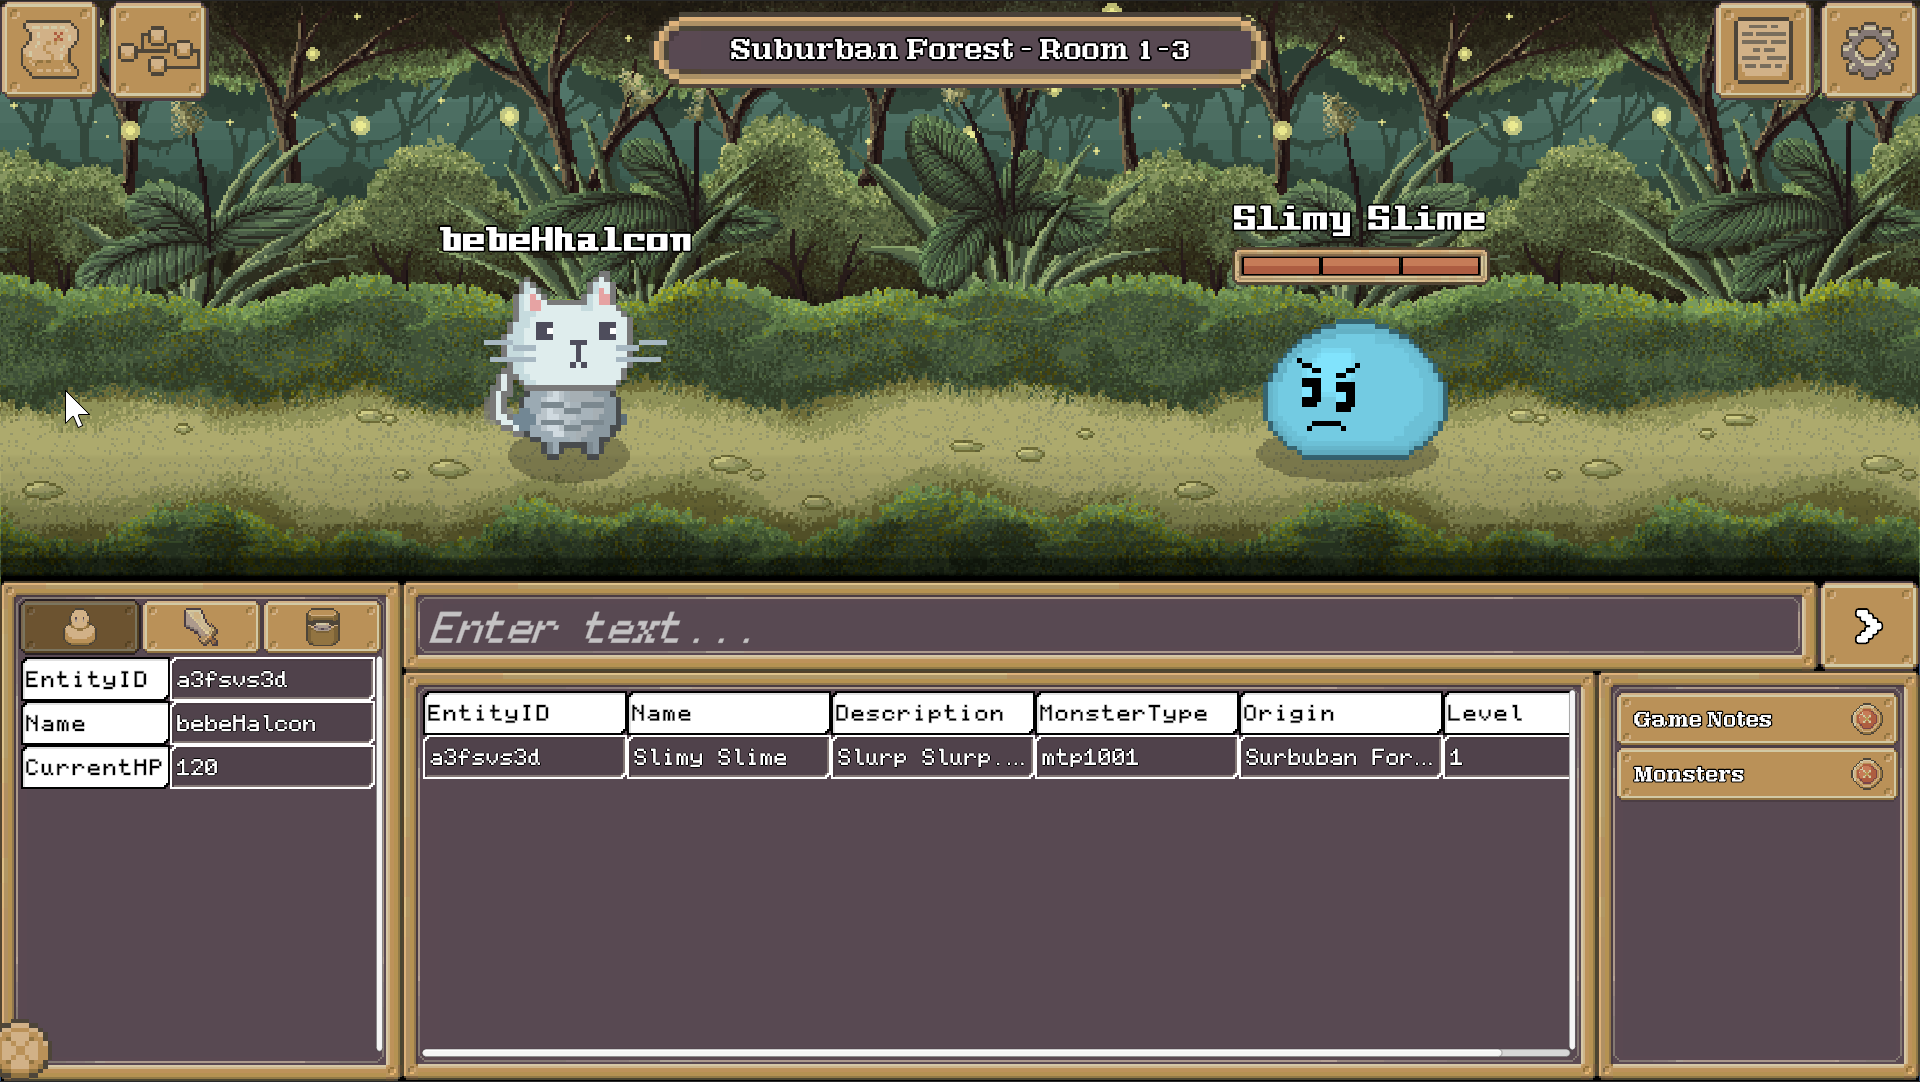
\includegraphics[width=\textwidth]{Images/Overall.png}
	\vspace{0.5cm}
	\caption{Tổng quan một màn chơi trong MeowSQL Knight}
\end{figure}
\hspace*{1cm} Người chơi sẽ sử dụng các câu truy vấn để khai thác schema cho sẵn. Sử dụng \textbf{select} để hiện nội dung các record lên màn hình, thu thập thông tin từ những dữ liệu đó. Ngoài ra cũng có thể \textbf{insert} và \textbf{delete} những record trên bảng và xem phản ứng của trò chơi sẽ như thế nào. Người chơi sẽ tấn công quái vật bằng các vũ khí mà người chơi mang vào trận chiến, tuy nhiên không thể tấn công quái vật một cách đơn thuần, người chơi sẽ phải tấn công vào các điểm yếu của quái vật nằm trên các bộ phận khác nhau. Để tương tác với game (tấn công quái vật, dùng vật phẩm), người chơi sẽ insert các tham số vào các bảng có chức năng đặc biệt, sau khi chèn xong thì hành động sẽ được thực thi.\\
\hspace*{1cm} Trong Schema này, các thực thể như người chơi, quái vật, bộ phận chí mạng của quái vật,... đều sử dụng chung ID có cấu trúc như nhau. Để tiêu diệt quái vật, người chơi phải nhắm đến các bộ phận chí mạng này, cũng như xác định được ID của chúng để có thể tấn công chính xác, bằng không các đòn đánh của người chơi sẽ bị trượt.\\
\hspace*{1cm} Người chơi phải tìm cách khai thác schema một cách hiệu quả trong chiến đấu. Đi kèm với việc lựa chọn trang bị hợp lý và tận dụng lợi thế môi trường, giành chiến thắng, hoàn thành màn chơi và đi sâu hơn để tìm ra bí ẩn của trò chơi.


\subsection{Sơ lược cốt truyện}
\hspace*{1cm} Trong một thế giới game RPG có chủ đề là động vật bình thường, bạn là một kỵ sĩ mèo đang đi rừng để tìm nguyên liệu, mọi thứ diễn ra một cách bình thường. \\
\hspace*{1cm} Đột nhiên, trò chơi bỗng hoạt động không đúng so với trước kia, các quái vật trở nên hung hãn hơn, nguy hiểm hơn, lẽ ra chỉ cần đánh bằng các phương pháp thông thường đã có thể diệt sạch chúng, nhưng kì lạ thay, các phương pháp thông thường không còn có hiệu quả với chúng nữa. Đám quái vật vùng lên làm loạn cả thế giới game, khiến thế giới game bị lỗi nghiêm trọng, và nếu cứ tiếp tục như vậy, trò chơi sẽ không thể chơi được nữa.\\
\hspace*{1cm} Chính lúc này, nhân vật chính của chúng ta bị một con slime bao vây, lẽ ra 1 nhát từ kiếm của cậu có thể hạ gục con Slime, tuy nhiên, trong thế giới game bị rối loạn như thế này là không thể. Cậu cứ đánh trong vô vọng, trong khi con quái vật giận dữ tiến gần định nuốt chửng cậu. Đột nhiên, một tia sáng xuất hiện giết chết con quái vật đó. Là Nhà phát triển (Dev) của trò chơi này. Anh ấy đã kiểm tra hệ thống thế giới game và phát hiện ra bạn là một trong những object hiếm hoi còn sống trong thế giới game này. Để hỗ trợ bạn, Dev cấp cho bạn 1 năng lực lớn: bạn có thể xem schema của game và thực hiện các câu truy vấn SQL để khai thác schema và chiến đấu. Vì chỉ có sử dụng SQL mới có thể đánh bại các quái vật SQL. \\
\hspace*{1cm} Dev muốn đặt niềm tin vào bạn vì Dev không thể khởi dộng lại Project game này, nó là một project chạy trên server nhưng cậu đã mất quyền kiểm soát cả server và project. Dev muốn bạn đi sâu vào bên trong lõi của game và tìm ra lý do khiến game trở nên như vậy. Bạn là hy vọng của thế giới game này, và là hy vọng của cả Dev. Bạn bắt đầu đi vào sâu trong thế giới, mang sứ mệnh vô cùng cao cả, không chỉ để cứu thế giới này.

\subsection{So Sánh các sản phẩm tương tự trên thị trường}
\hspace*{1cm} Nhắc đến dòng game giải đố theo lượt chúng ta không thể bỏ qua series game \textbf{Bookworm Adventures} được phát triển bởi \textit{\textbf{PopCap Games}}. Đây là một trong những trò chơi độc đáo kết hợp giữa ghép chữ và chiến đấu theo lượt, tạo ra phong cách riêng biệt và mới mẻ trong dòng game này.\\
\hspace*{1cm} Ở thời điểm hiện tại, trò chơi giải đố dựa trên cấu trúc của ngôn ngữ lập trình SQL đã xuất hiện trong một số sản phẩm. Sản phẩm nổi bật nhất là \textbf{SQL Murder Mystery} được phát triển bởi \textit{\textbf{Knight Lab}} của Đại học Northwestern, Mỹ.
\begin{figure}[H]
\centering
\begin{minipage}{.5\textwidth}
  \centering
  
\includegraphics[width=.5\linewidth]{Images/bookworm.jpg}
  \vspace{0.5cm}
  \caption{Bookworm Adventures}
  \label{fig:test1}
\end{minipage}%
\begin{minipage}{.5\textwidth}
  \centering
  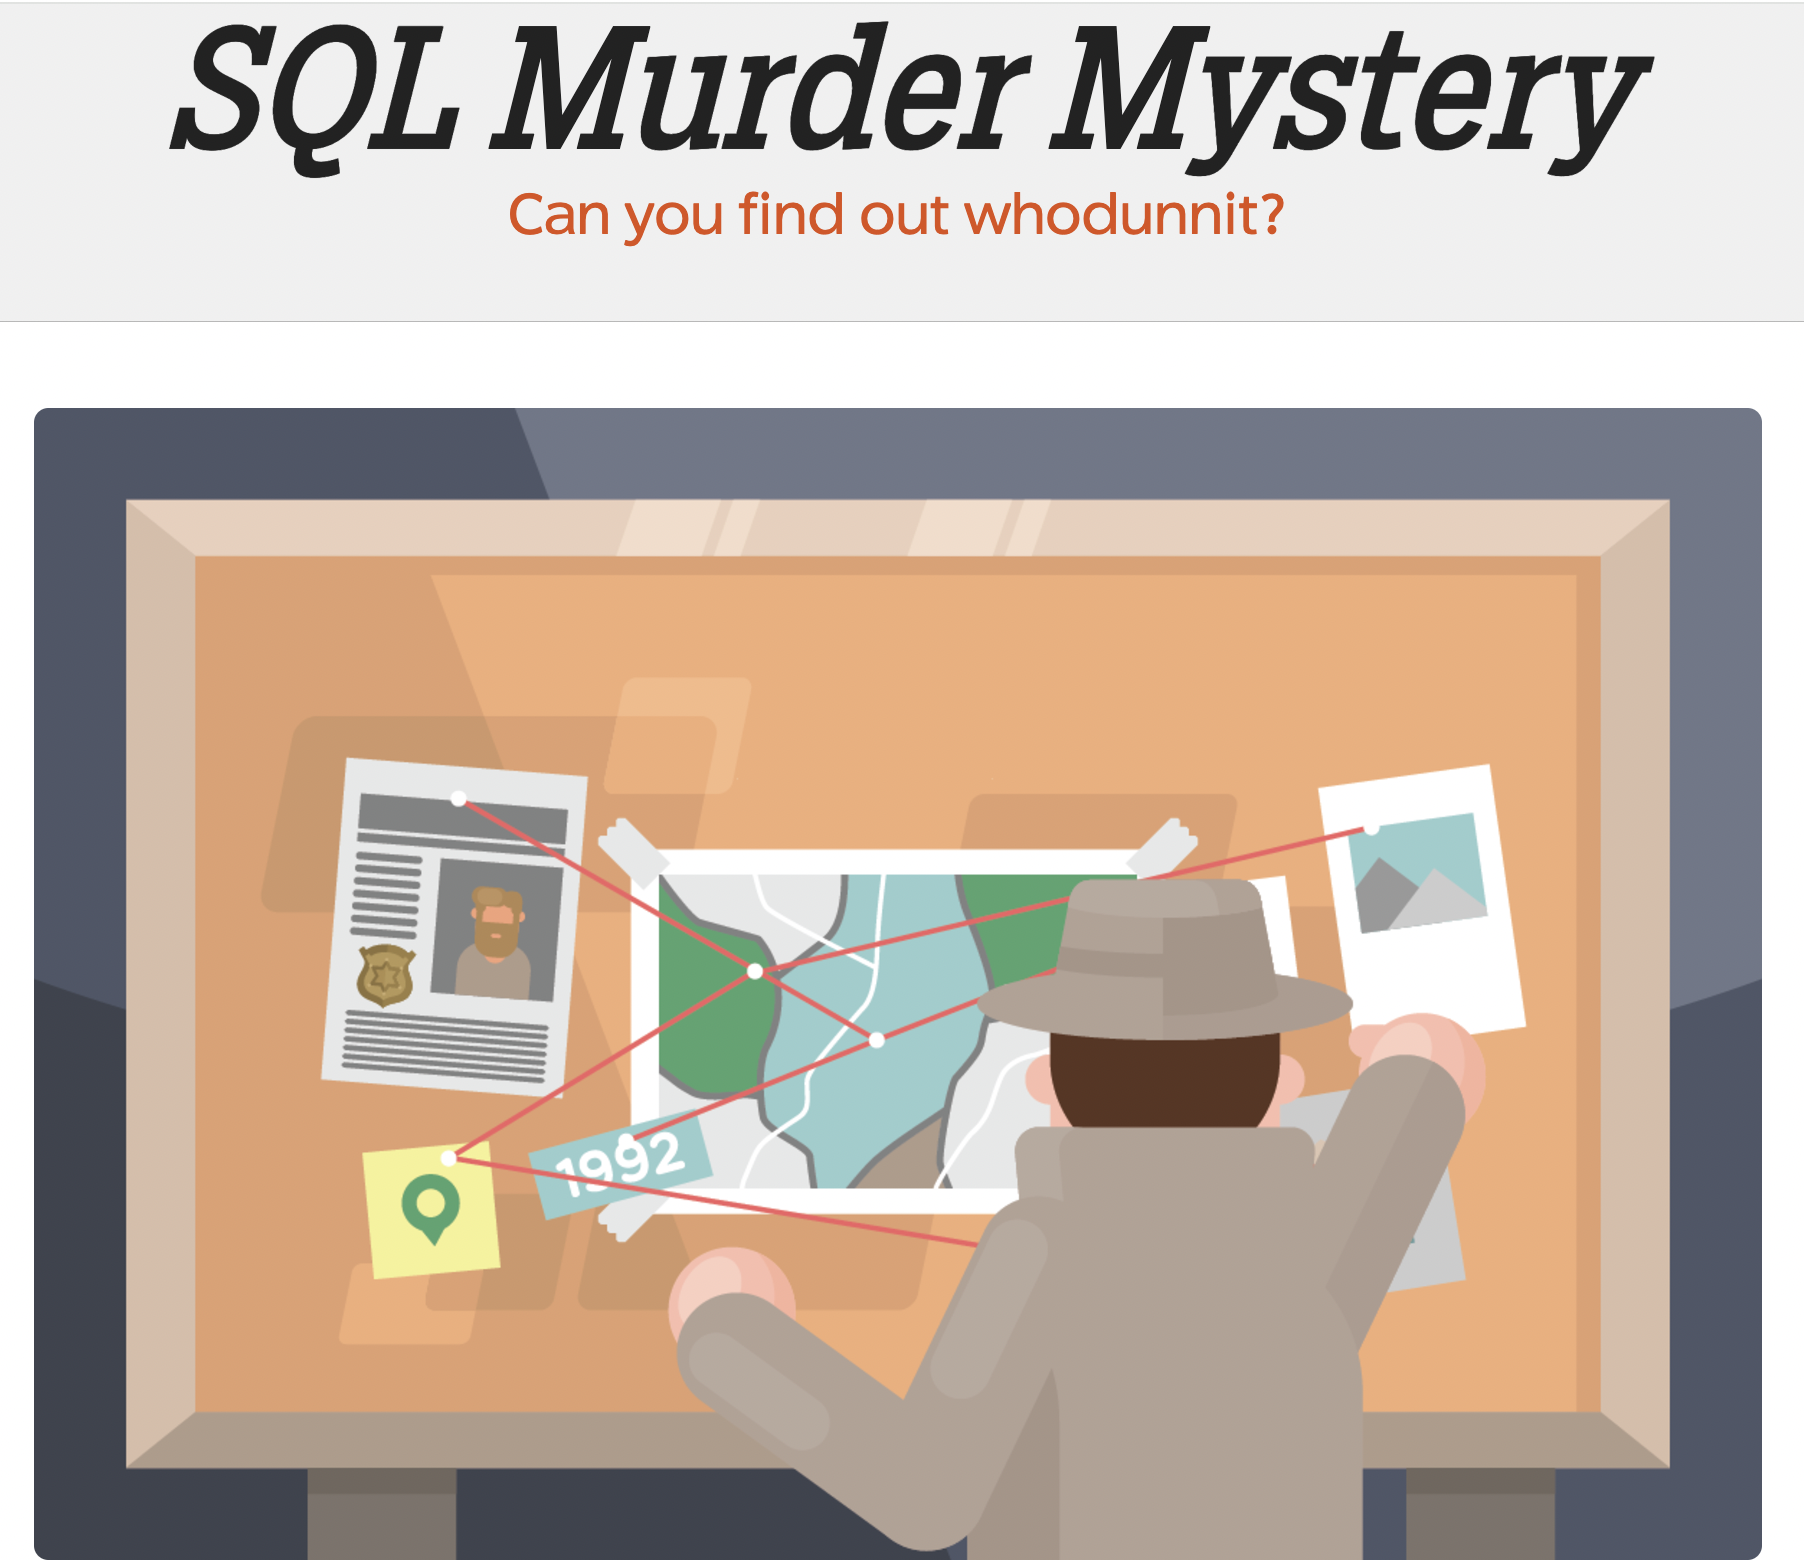
\includegraphics[width=.75\linewidth]{Images/SQL_murder.png}
  \vspace{0.5cm}
  \caption{SQL Murder Mystery}
  \label{fig:test2}
\end{minipage}
\end{figure}
\subsubsection{Bookworm Adventures}
\hspace*{1cm} Bookworm Adventures là một series game kết hợp giữa giải đố ghép chữ và yếu tố nhập vai chiến đấu. Người chơi điều khiển nhân vật chính, một chú sâu "mọt sách" Lex, trong hành trình phiêu lưu qua các thế giới thần thoại, đối đầu với quái vật và giải cứu bạn bè.\\
\hspace*{1cm} Người chơi sử dụng vốn từ vựng tiếng Anh để giúp Lex ghép các chữ cái trên màn hình thành các từ hợp lệ để tấn công quái vật bằng sức mạnh của từ ngữ. Từ càng dài và phức tạp thì sát thương gây ra càng cao.\\
\hspace*{1cm} Bookworm Adventures có hệ thống trang bị (mũ, vũ khí, phụ kiện) và dược phẩm để hỗ trợ Lex trong chiến đấu, ngoài ra còn có các chữ cái đặc biệt mang lại các hiệu ứng bổ sung (tăng sát thương, thiêu đốt, đóng băng..) khi được sử dụng để tạo từ.
\begin{figure}[H]
	\centering
	\includegraphics[width=0.75\textwidth]{Images/bookworm_play.png}
	\vspace{0.5cm}
	\caption{Tổng quan một màn chơi trong Bookworm Adventures}
\end{figure}
% \hspace*{1cm}
\subsubsection{SQL Murder Mystery}
\hspace*{1cm} SQL Murder Mystery là một trò chơi tương tác được thiết kế để giúp người chơi học và thực hành SQL thông qua việc giải quyết một vụ án bí ẩn. Chúng ta có thể chơi trực tuyến tại \def\UrlFont{\bfseries}\url{https://mystery.knightlab.com}, trò chơi hoàn toàn miễn phí và không yêu cầu cài đặt bổ sung.\\
\hspace*{1cm} Trong trò chơi, chúng ta sẽ sử dụng kĩ năng SQL của bản thân để truy bắt kẻ sát nhân đang lẫn trốn trong thành phố SQL. Trò chơi bắt đầu bằng việc khám phá một vài bảng dữ liệu, và dần dần, bạn sẽ phát hiện ra các manh mối liên quan đến vụ án mạng. Ví dụ, ngay từ đầu, bạn tìm thấy một báo cáo của cảnh sát đề cập đến hai nhân chứng nhưng không xác định được nghi phạm. Sau đó, bạn thực hiện JOIN với bảng phỏng vấn nhân chứng, và dần dần tiến gần hơn đến việc xác định tên tội phạm.
\begin{figure}[H]
	\centering
	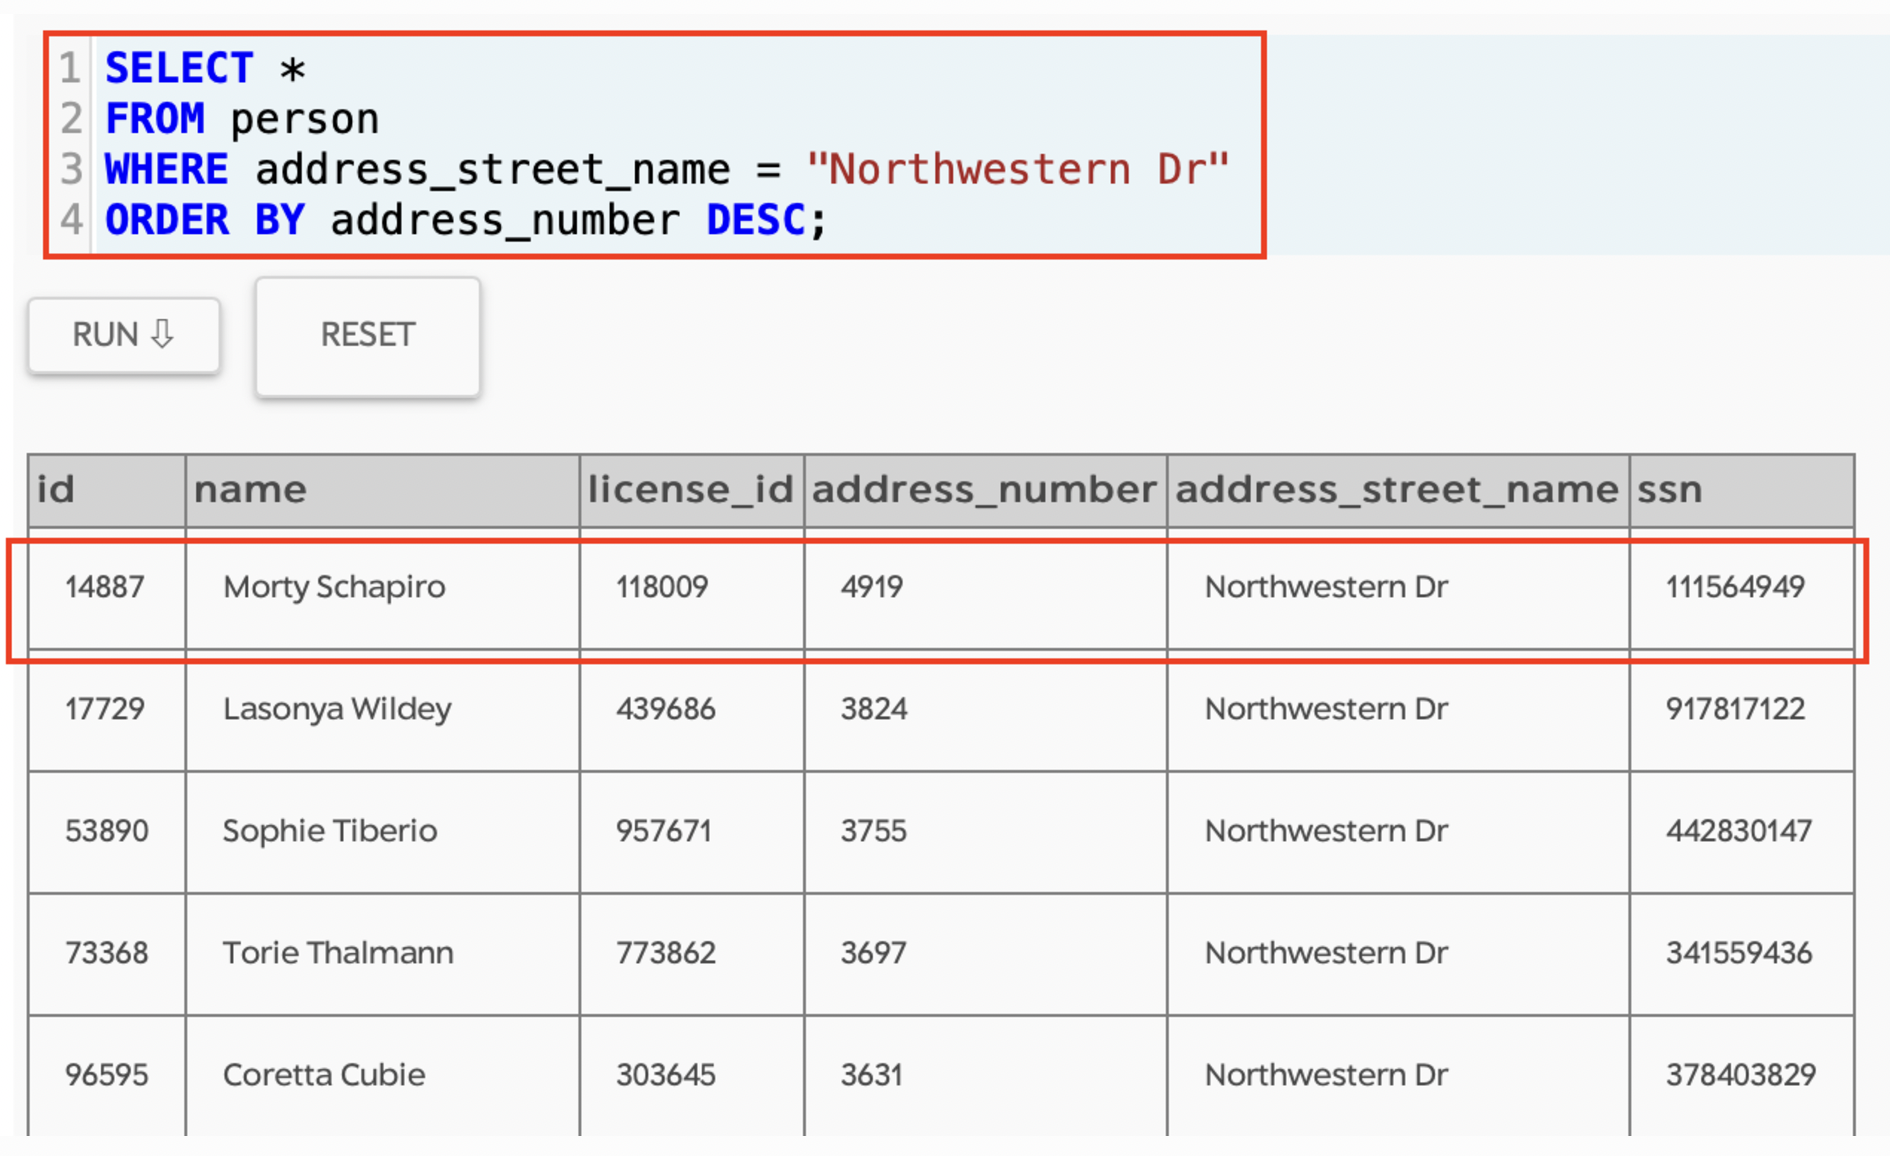
\includegraphics[width=0.75\textwidth]{Images/smm_play.png}
	\vspace{0.5cm}
	\caption{Tổng quan một câu truy vấn trong SQL Murder Mystery}
\end{figure}
\hspace*{1cm} Sau khi bắt được tên sát nhân ta nhận ra rằng hắn không phải kẻ chủ mưu thật sự. Các thám tử lại tiếp tục lên đường đi tìm tên thủ phạm đứng sau tất cả để trả lại trật tự cho thành phố SQL.
\begin{figure}[H]
\centering
\begin{minipage}{.5\textwidth}
  \centering
  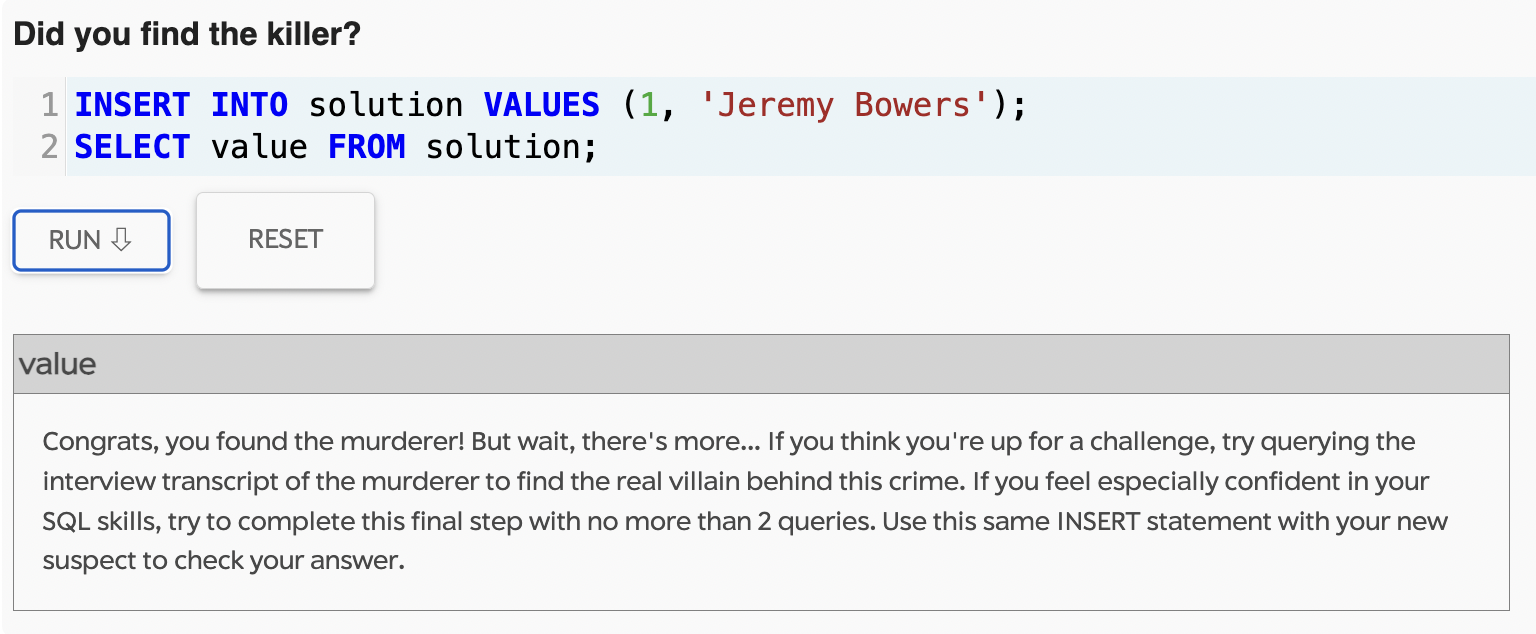
\includegraphics[width=0.75\linewidth]{Images/smm_killer.png}
  \vspace{0.5cm}
  \caption{Tìm ra kẻ sát nhân}
  \label{fig:test1}
\end{minipage}%
\begin{minipage}{.5\textwidth}
  \centering
  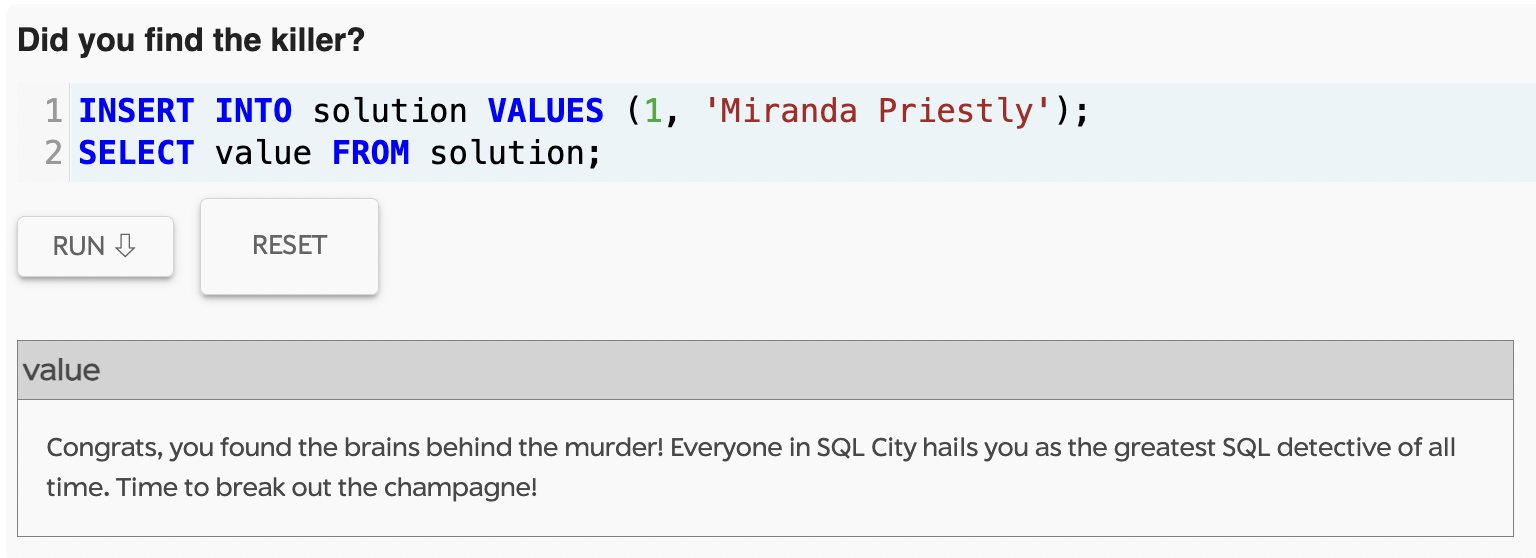
\includegraphics[width=.75\linewidth]{Images/smm_boss.png}
  \vspace{0.5cm}
  \caption{Tìm ra kẻ chủ mưu}
  \label{fig:test2}
\end{minipage}
\end{figure}
\hspace*{1cm} Trò chơi này đã nhanh chóng trở nên phổ biến nhờ cách tiếp cận sáng tạo và thú vị trong việc học lập trình SQL. Tuy nhiên, đồ hoạ của trò chơi vô cùng đơn giản, chỉ hiển thị kết quả của câu lệnh, không có hiệu ứng hay sự tương tác giữa game với người chơi. Nội dung của trò chơi cũng bị giới hạn quanh nhiềm vụ truy tìm thủ phạm, tính replay thấp.
\subsubsection{Điểm cải tiến của MeowSQL Knight}
\hspace*{1cm} Để MeowSQL Knight có thể tồn tài trên thị trường game, chúng ta cần khiến trò chơi có một nét riêng để thu hút người chơi đến với nó. Thông qua việc học tập, khắc phục những yếu điểm mà Bookworm Adventures và SQL Murder Mystery mắc phải và phát triển những tính năng mới. Trò chơi sẽ trở nên độc đáo, thu hút được một tập người chơi lớn hơn.\\
\hspace*{1cm} Đồ án kết hợp sử dụng ngôn ngữ truy vấn SQL vào chiến đấu theo lượt. Đồ án có giao diện Gameplay chính và xu hướng đồ hoạ slide scrolling giống với Bookworm Adventures. Trò chơi cũng có cốt truyện tập trung vào phiêu lưu và chiến đấu.
\subsection{Luật chơi}
\hspace*{1cm} Mỗi màn chơi, người chơi sẽ được đưa đến một bản đồ, gồm các phòng liên thông với nhau. Nhiệm vụ của người chơi là sử dụng các câu truy vấn để tương tác nhân vật chính, hoàn thành yêu cầu được đưa ra trong mỗi căn phòng, đến điểm cuối của bản đồ và hoàn thành màn chơi.

\subsection{Luật chơi Gameplay chính}
\hspace*{1cm} Mỗi màn chơi, người chơi sẽ được đưa đến một bản đồ, gồm các phòng liên thông với nhau. Nhiệm vụ của người chơi là sử dụng các câu truy vấn để tương tác nhân vật chính, hoàn thành yêu cầu được đưa ra trong mỗi căn phòng, đến điểm cuối của bản đồ và hoàn thành màn chơi.

\subsubsection{Bản đồ trong màn chơi}
\hspace*{1cm} Một màn chơi sẽ có dạng dungeon (hầm ngục) gồm nhiều phòng tại các tầng khác nhau, mỗi phòng có thể liên thông 1 chiều với nhau (có lối đi từ phòng này sang phòng khác nhưng không thể đi ngược lại) hoặc 2 chiều. Người chơi khi bắt đầu màn chơi sẽ bắt đầu ở căn phòng lối vào và kết thúc ở căn phòng lối ra. Chỉ có một lối vào và có một lối ra duy nhất. Ở lối ra thường sẽ có một Miniboss hoặc Boss trong đó. Các phòng bị bóng tối che khuất, chỉ có thể thấy các căn phòng lân cận (có lối đi từ phòng hiện tại) khi đã clear được căn phòng hiện tại.\\

\begin{figure}[H]
	\centering
	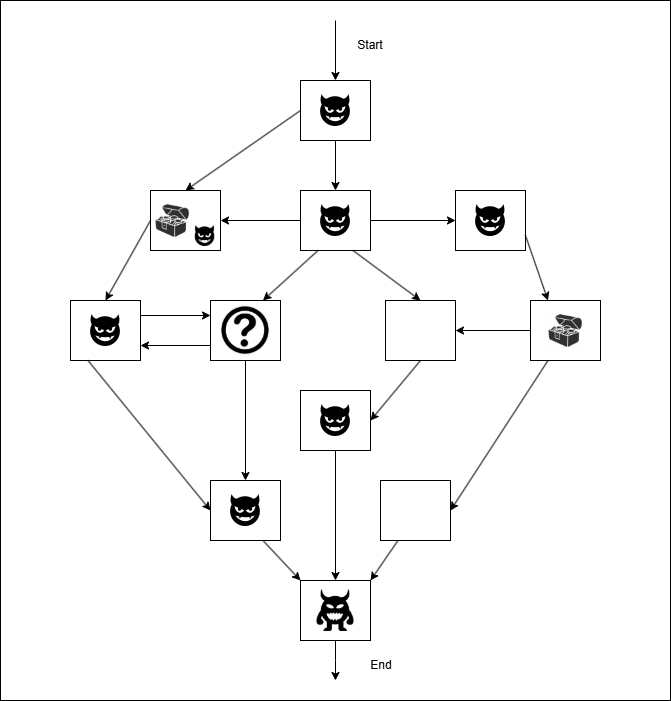
\includegraphics[width=10cm]{Images/SampleLevel.png}
	\vspace{0.5cm}
	\caption{Cấu trúc một bản đồ chơi}
\end{figure}

\hspace*{1cm}Trong một căn phòng, có thể xuất hiện quái vật, rương kho báu hoặc không có gì, đi cùng với một môi trường nhất định. Người chơi có thể chinh phục 1 căn phòng bằng các cách như tiêu diệt quái vật, mở rương kho báu hoặc đi vào 1 căn phòng trống. Sau khi chinh phục một căn phòng thì game sẽ mở khóa các căn phòng lân cận (không cần các phòng phải lối đi từ căn phòng hiện tại), người chơi quyết định đi căn phòng nào tiếp theo. Lưu ý rằng người chơi không được quay đầu (quay trở lại căn phòng đã đi trước đó). Các căn phòng có thể chứa các route đến các màn chơi khác trên bản đồ. Căn phòng cuối cùng, chính là lối ra, trong đó sẽ có một con boss hoặc min boss. Nhiệm vụ của người chơi là đánh bại boss đó để có thể thoát ra ngoài.\\
\subsubsection{Chiến đấu}
\hspace*{1cm}Gameplay chính của phần chiến đấu hoạt động theo dạng đánh theo lượt luân phiên giữa người chơi và quái vật.

\begin{itemize}
	\item Khi đến lượt của mình, người chơi được thực thi một câu lệnh hợp lệ của SQL. Câu lệnh phải chạy được thì mới tính là một câu lệnh hợp lệ. Để tấn công quái vật hoặc sử dụng vật phẩm, người chơi phải dùng câu \textbf{insert} để chèn các tham số vào các bảng mang chức năng đặc biệt. Mặc dù có cơ chế đánh theo lượt luân phiên, vẫn có khả năng người chơi sau khi xong một lượt có thể chơi một lượt nữa (đây gọi là sự nhanh nhẹn, nó sẽ là một chỉ số có ảnh hưởng đến xác suất đánh thêm lượt nữa của người chơi và quái vật). Để công bằng, cho dù người chơi có gia tăng chỉ số nhanh nhẹn cao bao nhiêu, xác suất tối đa để thêm lượt là 40\%. Điều này được tính cho cả quái vật. Tuy nhiên, mỗi thực thể chỉ có thể tấn công tối đa 2-3 lượt.
	\item Đến lượt của quái, Quái sẽ tấn công người chơi 1 lần duy nhất trong lượt, người chơi chắc chắn trúng đòn (sát thương có thể ít hay nhiều, thậm chí không đáng kể, không ảnh hưởng health). Đòn tấn công này có thể mang một số hiệu ứng khác nhau.
\end{itemize}

\subsubsection{Cơ chế đánh theo lượt}
\hspace*{1cm} Khi bắt đầu chiến đấu, lượt của thực thể được quyết định bằng một phép random với dải giá trị bao gồm điểm nhanh nhẹn của kẻ thù và người chơi, nếu random vào dải giá trị của đối tượng nào thì đối tượng đó được phép đi trước. Mỗi thực thể sẽ được cấp một chỉ số gọi là Turn Counter (TC) với giá trị ban đầu là độ nhanh nhẹn của thực thể đó. Đối với quái vật, nếu trong lượt quái vật tấn công người chơi thì TC sẽ bị giảm đi 70\% giá trị ban đầu, tương tự với player, nếu tấn công thì TC sẽ giảm 70\%, sử dụng vật phẩm thì giảm 60\%, chạy câu truy vấn hiển thị bảng ra màn hình thì giảm 60\%. Nếu TC về âm thì lượt tới sẽ là lượt của đối phương, ngược lại, việc quyết định lượt tiếp theo là của mình hay của đối phương sẽ phụ thuộc vào random tiếp với dải giá trị bao gồm TC còn lại của kẻ thù và người chơi. Nếu lượt tiếp theo là lượt của đối phương thì TC reset về chỉ số nhanh nhẹn (chưa tính trường hợp dính hiệu ứng độc, làm chậm, băng). Khi đến lượt của người chơi, nếu TC < 0 (do hiệu ứng băng) thì người chơi không thể thao tác và chuyển đến cuối lượt người chơi (nơi sẽ áp dụng hiệu ứng)\\
\subsubsection{Mã định danh thực thể}
\hspace*{1cm} Với một màn chơi, người chơi, quái vật và các bộ phận của nó sẽ được cấp một mã EntityID có cùng một định dạng, cấu trúc. Đây là chuỗi ký tự có độ dài 8 ký tự cố định (gồm số và chữ in thường và in hoa). Mỗi EntityID chỉ được sở hữu bởi nhiều nhất 1 object. Khi Object chết và màn chơi tiếp tục, EntityID này sẽ được thu hồi và nó không còn tồn tại với bất kỳ hình thức nào. Có một bảng lưu trữ các EntityID và loại Object được cấp phát.
\subsubsection{Người chơi}
\hspace*{1cm} Người chơi sẽ có một bảng trong schema để lưu trữ các thông tin khác nhau cần thiết cho việc chiến đấu với entityID thuộc về người chơi, các thuộc tính của người chơi tương tự với các Game RPG.\\
\begin{itemize}
	\item \textbf{Máu tối đa của người chơi} (base + current)
	\item \textbf{Máu hiện tại của người chơi}
	\item \textbf{Mô tả người chơi}
	\item \textbf{Màu sắc người chơi} (optional)
	\item \textbf{Sát thương cơ bản của người chơi} (base)
	\item \textbf{Nhanh nhẹn cơ bản}
	\item \textbf{Giáp của người chơi} (base + current)
	\item \textbf{Max slot trang bị}
	\item \textbf{EntityID của người chơi}
	\item \textbf{Level của người chơi}, có ảnh hưởng đến các chỉ số khác của người chơi, đồng thời ảnh hưởng khả năng sử dụng trang bị (giảm hoặc tăng)
\end{itemize}

\hspace*{1cm} Ngoài ra, người chơi được cung cấp một số lượng slot trang bị nhất định, người chơi trang bị vũ khí và giáp vào các slot này, mỗi slot chỉ được chứa một trang bị. Người chơi sẽ có môt inventory để chứa các vật phẩm và các trang bị không sử dụng. Trong chiến đấu, các vật phẩm tiêu hao sẽ được highlight và người chơi chỉ có thể được sử dụng chúng trong chiến đấu.
\subsubsection{Quái vật}
\hspace*{1cm} Mỗi quái vật có thông tin được lưu trữ trong 1 row của bảng Monster trong Schema. Các quái vật vẫn mang các chỉ số thuộc tính tương tự người chơi, tuy nhiên nó không có điểm máu (HP), vì vậy nó không tồn tại nhờ HP. Một số thuộc tính cơ bản:\\
\begin{itemize}
	\item \textbf{Tên quái vật}
	\item \textbf{Độ trà trộn}
	\begin{itemize}
		\item Thuộc tính trà trộn vào bảng thực thể và bảng monster.
		\item Một monster có thể có các bản sao làm hình nộm của nó và sẽ mang các EntityID riêng, chủ yếu để người chơi khó xác định được đâu mới là con thật mà tấn công (có thể gộp chung vào trí thông minh).
	\end{itemize}
	\item \textbf{Giáp cơ bản}: Bao gồm giáp và kháng hiệu ứng.
	\item \textbf{Màu sắc thân của quái vật}
	\item \textbf{Chủng loại quái vật}
	\item \textbf{Sát thương cơ bản: } Bao gồm sát thương thường, sát thương chí mạng và sát thương hiệu ứng
	\item \textbf{Nhanh nhẹn}
	\item \textbf{Nguồn gốc xuất xứ của quái vật}
	\item \textbf{Level}
	\item \textbf{Mô tả sơ bộ}
	\item \textbf{Phẩm chất (Traits):} mỗi quái vật sẽ có một phẩm chất, chủ yếu để chịu tác động từ môi trường.
\end{itemize}
\hspace*{1cm} Ngoài ra còn có các bảng liên quan đến Monster nhằm cung cấp gợi ý cho người chơi để xác định Entity của quái vật đúng.
\hspace*{1cm} Như đã nói ở trên, quái sẽ không sống nhờ HP, mà chúng sẽ sống nhờ vào các bộ phận chí mạng trên cơ thể, Tình trạng sống/chết của quái vật phụ thuộc vào tình trạng tồn tại của các bộ phận này. Nếu mất hết tất cả bộ phận chí mạng, quái sẽ chết. Quái cũng sẽ có một bộ kỹ năng, nhất định. Khi đến lượt của quái, quái sẽ chọn ngẫu nhiên một kỹ năng đã sẵn sàng và thi triển, kỹ năng nó cũng sẽ mất một khoảng thời gian để phục hồi. Các kỹ năng có đều mang một trait liên quan đến trait của bộ phận chí mạng. Nếu không có kỹ năng nào sẵn sàng để sử dụng, quái vật sẽ bỏ qua đợt tấn công.\\
\hspace*{1cm} Các bộ phận có thể nằm rải rác trên cơ thể và có EntityID tương tự với Quái vật và người chơi. Thông tin một bộ phận sẽ là một bảng ghi của bảng Monster Part chứa thông tin chung của tất cả bộ phận quái vật, bao gồm cả bộ phận ảo - bộ phận ngụy trang,… trong một level) trong Schema. Quái vật có thể có một số lượng bộ phận nhất định. Khi người chơi tấn công vào các bộ phận này, nếu nó không có chủ (hoặc chủ đã chết) sẽ được tính sát thương cao nhất (chưa trừ cộng về mặt khắc chế hoặc áp chế), ngược lại sẽ phải chịu giáp và kháng hiệu ứng của quái vật, rồi mới trừ vào máu của bộ phận, hiệu ứng sẽ áp dụng cho quái vật, người chơi vẫn tấn công vào EntityID của quái vật bình thường, nhưng hoàn toàn vô dụng, cả sát thương và hiệu ứng đều sẽ không áp dụng cho quái vật. Một số đặc điểm của một bộ phận. \\
\begin{itemize}
	\item \textbf{Máu tối đa}
	\item \textbf{Máu hiện tại}
	\item \textbf{Độ trà trộn}
	\begin{itemize}
		\item Thuộc tính trà trộn vào bảng thực thể và bảng Monster Part.
		\item Một monster có thể có các bản sao bộ phận làm hình nộm của nó và sẽ mang các EntityID riêng, chủ yếu để người chơi khó xác định được đâu mới là con thật mà tấn công. Chúng sử dụng trí thông minh để trà trộn các bộ phận ảo này vào. Các bộ phận này sẽ có máu bằng máu của bộ phận thật, tuy nhiên khi tấn công sẽ có xác suất 40\% bị huỷ diệt khi nhận sát thương. Một số bộ phận giả có thể đi kèm các hiệu ứng bẫy khi người chơi tiêu diệt các bộ phận này.
	\end{itemize}
	\item \textbf{Loại bộ phận} (tay súng, tay dao,…)
	\item \textbf{Phẩm chất (Traits):} mỗi bộ phận sẽ có tối đa 2 phẩm chất.
	\item \textbf{Nguồn gốc xuất xứ của quái vật}
	\item \textbf{Mô tả sơ bộ}
\end{itemize}
\hspace*{1cm} Ngoài ra còn có các bảng liên quan đến Monster Part (thường sẽ chung các bảng với Monster) nhằm cung cấp gợi ý cho người chơi để xác định Entity của quái vật đúng. Để có thể xác định EntityID chính xác, người chơi cần dựa vào tiếng kêu, các đặc điểm bề ngoài cũng như phản ứng đòn đánh và khi bị đánh của quái vật để nhận biết.
\hspace*{1cm} Quái sẽ tạo các bản sao Monster và Monster Part dựa trên độ trà trộn, độ trà trộn có thể ảnh hưởng đến số bản sao Monster, số bản sao Monster Part và độ giống với bản gốc (độ trà trộn càng cao thì record bản sao càng có xác suất giống bản gốc cao). Người chơi cần chú ý chỉ số này để có thể đưa ra các quyết định hợp lý.
\subsubsection{Hiệu ứng}
\begin{itemize}
	\item \textbf{Độc}
	\begin{itemize}
		\item Gây sát thương: 5\% lượng máu tối đa khi hết lượt
		\item Giảm độ nhanh nhẹn: 40\%
	\end{itemize}
	\item \textbf{Lửa}
	\begin{itemize}
		\item Gây sát thương: 15\% lượng máu tối đa khi hết lượt
	\end{itemize}
	\item \textbf{Băng}
	\begin{itemize}
		\item Giảm độ nhanh nhẹn xuống -1\%
	\end{itemize}
	\item \textbf{Làm chậm}
	\begin{itemize}
		\item Giảm độ nhanh nhẹn xuống 50\%
	\end{itemize}
	\item \textbf{Hiệu ứng câu lệnh}
	\begin{itemize}
		\item Người chơi không được sử dụng một từ khóa nhất định trong câu lệnh
	\end{itemize}
	\item \textbf{Mù}
	\begin{itemize}
		\item Người chơi sẽ không nhìn được một số ô trong bảng với câu \texttt{SELECT}
	\end{itemize}
\end{itemize}

\textbf{Chỉ số kháng hiệu ứng}
\begin{itemize}
	\item Mỗi người chơi/quái vật sẽ có một bộ chỉ số kháng hiệu ứng nhất định.
	\item Khi tấn công đối phương, nếu kháng hiệu ứng tương ứng lớn hơn sát lực hiệu ứng, đối phương sẽ không dính hiệu ứng.
	\item Nếu kháng hiệu ứng nhỏ hơn sát lực hiệu ứng, đối phương sẽ chịu hiệu ứng với trạng thái (state) của hiệu ứng cộng thêm sát lực hiệu ứng đó trừ cho kháng hiệu ứng.
	\item Trước khi kết thúc lượt của đối tượng hiện tại, hiệu ứng sẽ gây sát thương (nếu có) và trạng thái hiệu ứng được trừ đi một lượng chỉ số bằng kháng hiệu ứng của người chơi. Nếu trạng thái hiệu ứng nhỏ hơn hoặc bằng 0, hiệu ứng sẽ kết thúc.
\end{itemize}

\textbf{Trang bị và sát lực hiệu ứng}
\begin{itemize}
	\item Chỉ số kháng hiệu ứng của người chơi được tổng hợp từ nhiều trang bị trong slot.
	\item Mỗi món trang bị sẽ có một bộ sát lực riêng và không tính tổng hợp.
	\item Khi người chơi tấn công bộ phận nào của quái vật, sẽ tính sát lực hiệu ứng trên món trang bị và kỹ năng (skill) được sử dụng để tấn công.
\end{itemize}

\textbf{Hiệu ứng trên quái vật}
\begin{itemize}
	\item Quái vật sẽ chịu hiệu ứng trên thực thể của quái vật.
	\item Hiệu ứng sẽ gây sát thương lên bộ phận đó của quái vật.
\end{itemize}

\subsubsection{Trait System}
\hspace*{1cm} Có một bộ các Trait (phẩm chất) được sử dụng chung bởi các thực thể và trang bị. Mỗi object nói trên sẽ có một số lượng trait nhất định.\\
\hspace*{1cm} Trong hệ thống trait, Một trait có thể bị một hoặc nhiều trait khác khắc chế, hoặc một trait trait có thể khắc chế nhiều trait khác, cũng có thể không bị khắc chế hay khắc chế trait nào. Số lượng trait khắc chế không được vượt quá một ngưỡng nào đó. Hệ thống trait sẽ luôn được điều chỉnh bởi người thiết kế màn chơi, người thiết kế phải cố gắng giữ cho các trait được cân bằng, không có trait nào quá mạnh, quá yếu.\\ 
\hspace*{1cm} Quái vật sẽ có 1 trait, chịu khắc chế của môi trường (bản thân môi trường cũng có một trait, chủ yếu gây khắc chế và áp chế) ảnh hưởng đến đòn đánh, Bộ phận của quái cũng có tối đa 2 trait, chịu khắc và áp chế từ sát thương vũ khí người chơi.
\subsubsection{Cơ chế kho đồ/trang bị}
Thứ cần thiết cho game không thể thiếu là các vật phẩm, các trang bị sẽ hỗ trợ người chơi trên chuyến hành trình. Các vật phẩm có thể có nhiều cách thu thập khác nhau:
\begin{itemize}
	\item Thu thập khi mở rương trong màn chơi
	\item Thu thập qua đánh boss
	\item Mua bán, trao đổi
	\item Gacha
	\item Ghép vật phẩm
\end{itemize}

Các vật phẩm sẽ có các thuộc tính khác nhau, và có các công dụng khác nhau giúp người chơi có thể lựa chọn.

\textbf{Phân cấp theo độ hiếm}
Việc phân cấp này chủ yếu diễn ra ở trang bị, có thể chia thành các phân cấp như sau:
\begin{itemize}
	\item Common
	\item Uncommon
	\item Rare
	\item Super-Rare
	\item Myth
	\item Legendary
\end{itemize}

Mỗi phân cấp khác nhau sẽ mở khóa tiềm năng trang bị khác nhau, bao gồm chỉ số cơ bản, giới hạn chỉ số tối đa, các skill độc quyền,...

Đối với các item tiêu thụ được, kích thước của chúng phụ thuộc vào 3 độ hiếm: 
\begin{itemize}
	\item Common (nhỏ)
	\item Uncommon (vừa)
	\item Rare (lớn)
\end{itemize}
Độ hiếm càng cao giới hạn chỉ số càng lớn, ngoài ra còn đi kèm các hiệu ứng mạnh hơn, cũng như nhiều traits hơn (giới hạn tối đa 5 traits)
\textbf{Các chỉ số trang bị}
Trang bị vũ khí và trang bị giáp đều mang một bộ chỉ số cố định, phù hợp cho việc hiện thực cũng như cho việc khi combat, người chơi có thể sử dụng giáp để chiến đấu.
\begin{itemize}
	\item Chỉ số cơ bản
	\item Phẩm chất (Traits)
	\begin{itemize}
		\item tấn công cơ bản
		\item giáp cơ bản
		\item nhanh nhẹn
		\item kháng hiệu ứng
		\item hút máu
		\item phản đòn
		\item hồi máu mỗi lượt
		\item ...
	\end{itemize}
	\item Giới hạn chỉ số
	\begin{itemize}
		\item tấn công tối đa
		\item giáp tối đa
		\item kháng hiệu ứng tối đa
	\end{itemize}
	\item Nâng cấp
	\begin{itemize}
		\item Hệ số nâng cấp giáp
		\item Hệ số nâng cấp vũ khí
	\end{itemize}
	\item Ảnh hưởng của Level người chơi
	\begin{itemize}
		\item Level yêu cầu
		\item Mức giảm stat nếu dưới level
	\end{itemize}
\end{itemize}

\textbf{Các loại trang bị}
\begin{itemize}
	\item Vũ khí
	\begin{itemize}
		\item Vũ khí dùng để tấn công quái vật cho ra sát thương tốt nhất, mỗi loại vũ khí khác nhau sẽ có bộ kỹ năng khác nhau.
	\end{itemize}
	\item Giáp
	\begin{itemize}
		\item Khi quái vật tấn công vào giáp thì giáp sẽ phát huy hiệu quả khi ngăn cản đòn đánh của quái vật cũng như có thể kháng hiệu ứng. Người chơi vẫn có thể tấn công quái vật bằng giáp được, nhưng sát thương của chúng thường rất nhỏ.
	\end{itemize}
	\item Giày
	\begin{itemize}
		\item Giày có thể tăng chỉ số giáp và nhanh nhẹn, cũng như giáp, chỉ số tấn công gần như bằng 0 nên Khi quái vật tấn công vào thì giáp sẽ phát huy hiệu quả khi ngăn cản đòn đánh của quái vật cũng như có thể kháng hiệu ứng.
	\end{itemize}
	\item Kỹ năng (Chiêu)
	\begin{itemize}
		\item Mỗi món trang bị có một chiêu nhất định, giúp khuếch đại đòn đánh cũng như đi kèm với các hiệu ứng khác nhau, chủ yếu là lửa, độc, băng,...
		\item Một số thông số của chiêu cơ bản:
		\begin{itemize}
			\item Hệ số khuếch đại sát thương
			\item Hệ số khuếch đại giáp cơ bản
			\item Hệ số khuếch đại nhanh nhẹn
			\item Hệ số hút máu
			\item ...
		\end{itemize}
	\end{itemize}
	\item Khi sử dụng vũ khí có trait tấn công bộ phận quái vật, ta sẽ xét tổng số cặp khắc chế và tổng số cặp bị khắc chế của vũ khí sử dụng. Nếu số cặp khắc chế lớn hơn thì xem như đòn đánh có lợi thế về khắc chế.
	\item Về giáp và giày có nhiều trait, trait tổng quan của player được tính là hợp của tập các trait của từng trang bị. Nếu số trait lớn hơn 5, thì trang bị đứng trước sẽ được ưu tiên về trait hơn.
\end{itemize}
\textbf{Cơ chế Kho đồ/ Slot trang bị}
\begin{itemize}
	\item Kho đồ trong game có không gian lưu trữ lớn, nhưng nó có giới hạn, chủ yếu lưu trữ các trang bị không sử dụng và các vật phẩm tiêu hao cùng vật phẩm khác. Khi người chơi chết thì tất cả các món đồ trong kho không bị ảnh hưởng.
	\item Slot trang bị cho phép người chơi gán các trang bị vào để mang đi chiến đấu. Có tối đa 8 slot trang bị, ban đầu người chơi chỉ có 4 slot trang bị, có thể nâng cấp tại cửa hàng. Nếu người chơi chết, các món trang bị không bị mất, nhưng chúng sẽ bị giảm cấp độ (tùy dev tùy chỉnh mà có thể giảm ít, hay nhiều).
	\item Trong màn chơi, người chơi không được gán trang bị từ kho vào slot và ngược lại. Việc này chỉ được thực hiện bên ngoài bản đồ hay ở khu Safe Zone.
\end{itemize}
\subsubsection{Môi trường}
\textbf{1cm} Mỗi căn phòng trong màn chơi có một môi trường tương ứng. Có một bảng gồm ID phòng, một mã môi trường trong căn phòng đó, cùng với thuộc tính (trait) của môi trường. Các vật phẩm, quái vật sẽ chịu ảnh hưởng của môi trường theo hướng mạnh hơn, yếu đi hoặc không bị ảnh hưởng tương ứng với mã môi trường. Mã môi trường là cố định.\\

\textbf{Vật thể trong môi trường}
\textbf{1cm} Ngoài ID môi trường trong phòng, mỗi phòng sẽ có một bảng tên là Environment Object chỉ các vật thể trong môi trường. Các vật thể sử dụng EntityID làm khóa chính tương tự với các object khác. Ngoài ra còn có mô tả được sinh bởi hệ thống game, giúp người chơi thu thập các manh mối tạo lợi thế trong màn chơi. Bảng này người chơi có thể thêm và xóa các record khác nhau. Tuy nhiên, cần cẩn thận vì một số vật thể nếu xóa đi sẽ gây bất lợi cho người chơi, thậm chí còn có thể giết người chơi ngay lập tức.\\

\hspace*{1cm} Các vật thể này có thể được sử dụng làm vũ khí để tấn công, nếu nó được xem là có thể gây sát thương (ví dụ như dao từ quái vật phi dao). Nếu không, khi tấn công, game sẽ thông báo rằng object người chơi chọn để tấn công không có gì xảy ra sau đó.\\

\subsubsection{Cơ chế gõ lệnh}
\hspace*{1cm}Người chơi chỉ được gõ lệnh khi đến lượt của mình, Ngôn ngữ truy vấn người chơi sử dụng là SQL, thuộc dạng Declarative Language. Người chơi chỉ được thực hiện 1 câu lệnh, nếu người chơi cố tình nhập nhiều câu lệnh trong một lượt thì game sẽ thực thi câu lệnh đầu tiên được nhập vào và hủy toàn bộ các câu lệnh sau (đồng thời nhắc nhở người chơi về hành động này).\\
\hspace*{1cm} Người chơi có thể sử dụng các câu truy vấn \texttt{SELECT} để lấy thông tin của một bảng trong schema, một bảng người chơi tự tạo,... Người chơi có thể chèn giá trị, cập nhật giá trị và xóa giá trị cho bảng đó cho mục đích khác nhau.\\
\hspace*{1cm} Người chơi sử dụng schema để xác định EntityID phù hợp để tấn công. Muốn tấn công quái vật người chơi cần chèn vào bảng Attack với các giá trị 
\begin{verbatim}
	(EntityID target, ItemID equipment, [optional] SkillID skill)
\end{verbatim}
Trong đó:
\begin{itemize}
	\item \textbf{target}: EntityID mục tiêu cần tấn công, mục tiêu có thể là của quái vật, của bộ phận và cả của người chơi.
	\item \textbf{equipment}: ID trang bị sử dụng để tấn công (vấn đề này sẽ được nói trong phần sau), ID này phải là của item nằm trong slot trang bị. Trang bị tấn công có thể là giáp và vũ khí.
	\item \textbf{skill}: là mã của chiêu thức tương ứng với vũ khí, (có thể thay bằng index cho tiện). Mỗi trang bị sẽ có một số chiêu thức nhất định, người chơi có thể lựa chọn chiêu thức, cũng như tham khảo chúng từ bảng trong schema. Người chơi có thể tấn công bằng đánh thường (không nhập index chiêu).
\end{itemize}

Ngoài ra, người chơi có thể sử dụng các vật phẩm tiêu hao để hỗ trợ trong chiến đấu bằng cách chèn giá trị vào bảng Use với giá trị:
\begin{verbatim}
	(ItemID item)
\end{verbatim}
trong đó \texttt{item} là vật phẩm tiêu hao được trong inventory, các item này sẽ hiện lên đầu tab Inventory và sẽ được highlight để người chơi nhận biết.
\subsubsection{Win condition}
Người chơi sẽ thắng khi đánh bại được quát vật, tức là khiến cho hp của nó về 0.
\subsubsection{Lose condition}
Người chơi sẽ thua khi bị tiêu diệt bởi quái vật, để hp của mình chạm đến 0.
\subsection{Các đối tượng chính trong màn chơi}
\subsubsection{Người chơi}
\begin{figure}[H]
	\centering
	
\includegraphics[width=5cm]{Images/Player.png}
	\vspace{0.5cm}
	\caption{Người chơi}
\end{figure}
\subsubsection{Quái vật}
\begin{figure}[H]
	\centering
	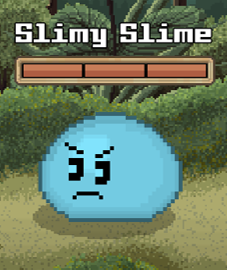
\includegraphics[width=5cm]{Images/Monster.png}
	\vspace{0.5cm}
	\caption{Quái vật}
\end{figure}
\subsubsection{Thông số, trang bị và kho đồ}
\begin{figure}[H]
	\centering
	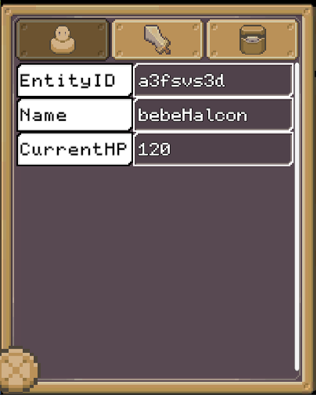
\includegraphics[width=10cm]{Images/Inventory.png}
	\vspace{0.5cm}
	\caption{Thông số, trang bị và kho đồ}
\end{figure}
\subsubsection{Ô nhập lệnh và kết quả truy vấn}
\begin{figure}[H]
	\centering
	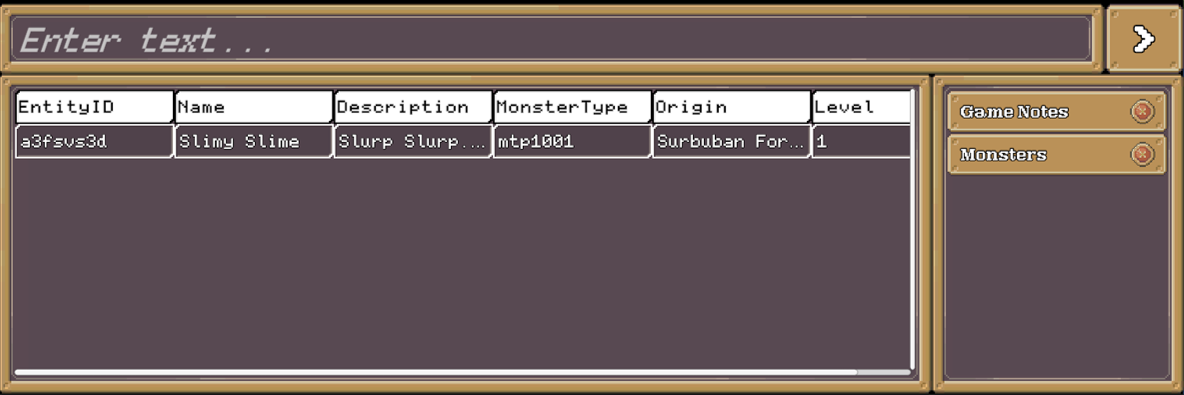
\includegraphics[width=10cm]{Images/CommandBox.png}
	\vspace{0.5cm}
	\caption{Ô nhập lệnh và kết quả truy vấn}
\end{figure}
\subsubsection{Bản đồ màn chơi và phòng hiện tại}
\begin{figure}[H]
	\centering
	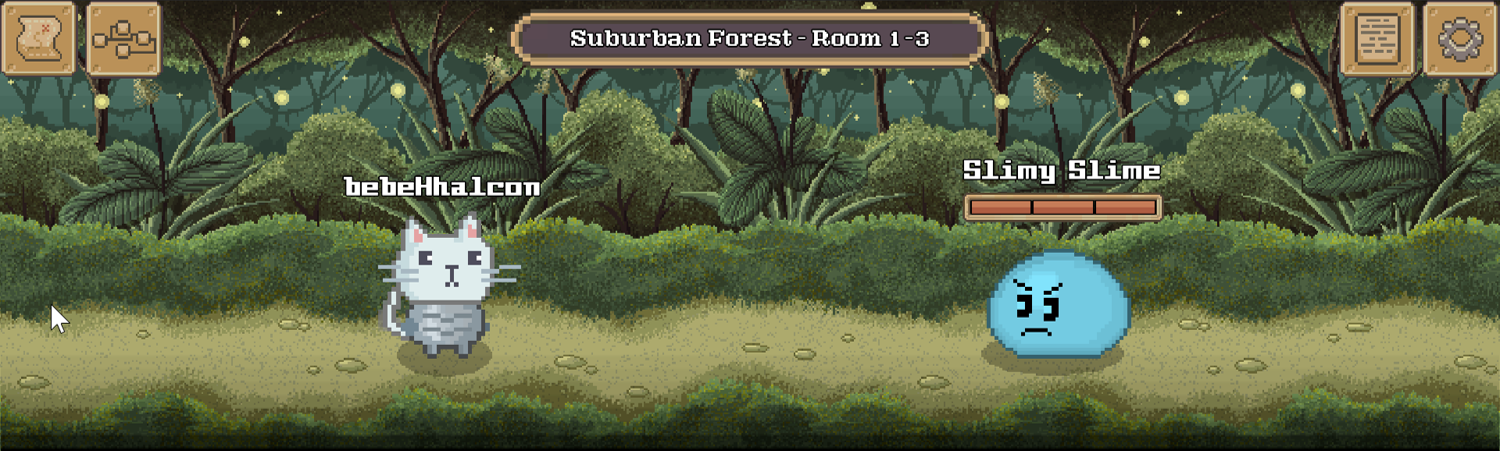
\includegraphics[width=10cm]{Images/CurrentRoom.png}
	\vspace{0.5cm}
	\caption{Quang cảnh môi trường của phòng chơi hiện tại}
\end{figure}

\newpage
\section{Cơ sở lý thuyết}
\subsection{Phát triển trò chơi}
\hspace*{0.5cm} \textit{Video game (hay trò chơi điện tử)} là trò chơi được vận hành bằng các thiết bị điện tử để tạo môi trường tương tác. Trải qua các giai đoạn lịch sử, với sự phổ biến và phát triển của công nghệ, trò chơi điện tử ngày càng phổ biến với người dùng hơn. Các máy, hay còn gọi là “nền tảng,” mà trên đó trò chơi điện tử được chơi có thể là máy tính cá nhân, máy game arcade (game thùng), máy chơi game kết nối với tivi gia đình, máy chơi game cầm tay, thiết bị di động như điện thoại di động, máy tính bảng,... với đủ mọi thể loại như casual, giải đố, các game double A hoặc triple A,...\\
\hspace*{0.5cm} \textit{Phát triển trò chơi điện tử} là một  quá trình sáng tạo, kết hợp các yếu tố nghệ thuật như thiết kế, đồ hoạ, âm thanh, hình ảnh và các yếu tố kỹ thuật như cấu trúc dữ liệu, xử lý đầu vào, thuật toán, AI,... để tạo ra một trò chơi điện tử. Quá trình này trải qua nhiều công đoạn khác nhau:\\
\begin{itemize}
	\item \textbf{Lên kế hoạch}: Nghiên cứu thị trường, xác định thể loại và concept chỉnh của trò chơi, mục đích và lên kế hoạch cho các cột mốc cho dự án.
	\item \textbf{Tiền sản xuất}: Khi ý tưởng đã được hình thành và kế hoạch đã được vạch ra rạch ròi thì giai đoạn này là giai đoạn dành cho việc thiết kế và hình thành nên cơ chế và thế giới game về mặt ý tưởng. Đây là bước rất quan trọng, có thể ảnh hưởng trải nghiệm chơi game về sau.
	\item \textbf{Sản xuất}: Đây là phần quan trọng nhất của quá trình, là quá trình tốn rất nhiều thời gian để thực sự tạo ra trò chơi điện tử theo từng thành phần phần và kết hợp chúng lại với nhau. Bước này cũng có thể là phần khó khăn nhất vì có thể phát sinh các vấn đề cần được giải quyết, trong khi một số yếu tố của trò chơi có thể phải bị cắt bỏ hoặc thay đổi. Điều này có thể kéo dài một vài tuần hoặc tháng cho thời gian phát triển.
	\item \textbf{Kiểm thử}: Khi phiên bản đầu tiên của trò chơi đã được sản xuất. Trò chơi phải được kiểm tra kỹ lưỡng để phát hiện bất kỳ vấn đề nào trong thiết kế trò chơi hoặc code có thể khiến trò chơi không hoạt động đúng cách. Debug giúp phát hiện và sữa chữa sự cố trong mã nguồn trò chơi. Nó cũng có thể làm phát sinh các vấn đề lớn hơn khi thiết kế trò chơi không hoạt động như dự kiến – ví dụ, một người chơi có thể phá vỡ trò chơi bằng cách tiếp cận các khu vực không được phép một cách không đúng.Kiểm tra không chỉ để tìm các vấn đề cụ thể. Nó cũng có thể đánh giá cảm giác tổng thể của trò chơi. Ví dụ, trò chơi có quá dễ hay quá khó không? Câu chuyện có lôi cuốn không? Kiểm tra có thể giúp trả lời những câu hỏi này.
	\item \textbf{Tiền phát hành}: Đến thời điểm này, trò chơi đã được phát triển thành một sản phẩm gần như sẵn sàng để phát hành. Một phiên bản beta của trò chơi có thể được gửi cho một số ít người chơi được chọn để nhận phản hồi và giúp xác định những thay đổi vào phút chót.Thời gian trước khi ra mắt cũng là lúc thực hiện các hoạt động marketing và quảng cáo thông qua trailer và áp phích, và các studio AAA sẽ trình bày một cách thu hút tại các hội chợ trò chơi. Phiên bản sớm của trò chơi có thể được gửi đến các nhà phê bình tại các tạp chí trò chơi và những chuyên gia khác, những người sẽ chơi trò chơi và đánh giá, sau đó được công bố trực tuyến.Các bài đánh giá có thể giúp tạo sự hứng thú nếu trò chơi được đánh giá cao, nhưng không đảm bảo sẽ phù hợp với quan điểm của cộng đồng game thủ rộng lớn. Có một số trường hợp trò chơi bị các chuyên gia cho điểm thấp nhưng cộng đồng game thủ lại đánh giá cao.
	\item \textbf{Phát hành}: Giai đoạn ra mắt bao gồm việc sửa các lỗi còn sót lại trong trò chơi để đảm bảo trò chơi sẵn sàng cho việc phát hành rộng rãi. Một số cải tiến nhỏ cũng có thể được thêm vào để hoàn thiện sản phẩm cuối cùng.
	\item \textbf{Hậu phát hành}: Sau khi phát hành, có thể xuất hiện các lỗi. Việc sửa lỗi là điều không thể tránh khỏi khi số lượng người chơi trò chơi (hy vọng) sẽ gặp phải các vấn đề. Việc sửa chữa các lỗi này càng sớm càng tốt thông qua các bản cập nhật là điều cực kỳ quan trọng để đảm bảo khách hàng có thể tận hưởng trò chơi và tạo ảnh hưởng tốt trong cộng đồng. Ngoài ra, trong giai đoạn hậu ra mắt, công việc vẫn có thể tiếp tục để tạo thêm nội dung cho trò chơi nhằm giữ chân người chơi. Nội dung bổ sung này thường được phát hành dưới dạng các bản cập nhật lớn theo mùa hoặc DLC (Downloadable Content - nội dung có thể tải xuống) đóng vai trò như một phần mở rộng cho game gốc. Quá trình phát triển nội dung mới có thể làm giai đoạn phát triển quay trở lại giai đoạn lên kế hoạch (cho các nội dung mới).
\end{itemize}
\subsection{Thiết kế màn chơi}
\hspace*{0.5cm} Một màn chơi là không gian những gì cốt lõi diễn ra trong game. Nơi này đặt ra những giới hạn cho người chơi trong việc tương tác với game. Có sự đa dạng trong từng level. Mỗi level có thể có một số điểm tương đồng, nhưng mỗi màn sẽ có những nét đặc trưng khác nhau.\\
\hspace*{0.5cm} Thiết kế màn chơi là một giai đoạn của quá trình phát triển trò chơi nơi các nhà phát triển tập trung tạo ra các không gian này, bao gồm các cấp độ, bản đồ và nhiệm vụ trong game. Việc thiết kế trò chơi là việc kết hợp các yếu tố cấu thành nên trải nghiệm người chơi, bao gồm cơ chế game, gameplay, cốt truyện,...\\
\hspace*{0.5cm} Tuy nhiên, việc thiết kế màn chơi không phải để cho có. Việc thiết kế màn chơi cần có một mục đích nào đó, ví dụ như kể chuyện, có nhân vật và phục vụ cho mục đích rõ ràng trong game. Hơn hết, người thiết kế phải tập trung vào trải nghiệm người chơi, hơn là cảm nhận bản thân. Và màn chơi phải thực sự cuốn hút và vui để mang đến trải nghiệm cho người chơi\\
\hspace*{0.5cm} Mục tiêu của việc thiết kế màn chơi là tạo ra các sự kiện tương tác trong môi trường game sao cho chúng mang tính thử thách người chơi. Giúp người chơi đạt được cảm giác vui sướng khi hoàn thành và có mong muốn tiếp tục gắn bó với game.\\
\subsubsection{Các bước thiết kế một màn chơi}
\hspace*{0.5cm} Để thiết kế màn chơi, cần tập trung vào các bước chính sau:
\begin{enumerate}
	\item \textbf{Xác định lại giới hạn dự án}\\
	Các ý tưởng có thể có rất nhiều, trông chúng có thể rất hay nhưng mà ta cũng nên nhìn lại xem giới hạn của dự án có phù hợp cho ý tưởng này không, từ đó chọn được các ý tưởng phù hợp. Nó có thể đến từ bản chất của dự án hoặc kỹ thuật. Người thiết kế màn chơi cần hiểu rõ các giới hạn này để thiết kế màn chơi sao cho hợp lý.\\
	\hspace*{0.5cm} Về bản chất của dự án. Điều cần phải chú ý nhất là người chơi cũng như nền tảng hiện thực. Ta cần xác định đối tượng người chơi chủ đạo của game (là trẻ em, người trưởng thành hay người cao tuổi, là nam hay nữ, có phải là mẹ bỉm sữa hay không,...) cũng như nền tảng để chơi (mobile, PC hay console). Điều này ảnh hưởng đến thời gian hoàn thiện, độ dài và độ khó của màn chơi cũng như phong cách đồ hoạ. Những dự án làm trên mobile sẽ nhanh hơn so với PC hay console. Những trò chơi nhắm đến đối tượng trẻ em thì độ dài màn chơi sẽ ngắn, độ khó cũng dễ hơn cũng như phong cách đồ hoạ cũng sẽ nhẹ đô hơn so với các game dành cho lứa tuổi người trưởng thành. Ta không thể sản xuất một tựa game có phong cách đồ hoạ máu me, hoặc chủ đề có liên quan đến chiến tranh cho đối tượng là trẻ em được.\\
	\hspace*{0.5cm} Về vấn đề kỹ thuật, người thiết kế màn chơi phải giữ cho game có tính nhất quán về mặt công nghệ. Người thiết kế cần biết dự án sẽ sử dụng công nghệ nào, phong cách đồ hoạ ra sao, âm thanh, nhạc nền như thế nào. Một trò chơi không thể sử dụng lẫn lộn đồ hoạ pixel và đồ hoạ vector nếu không có mục đích cụ thể, hoặc có mục đích nhưng sử dụng không hợp lý. Một trò chơi về chiến tranh thế giới thời hiện đại không thể xuất hiện các yếu tố như pháp sư, phù thuỷ hay kiếm sĩ trong các tựa game RPG được. Ngược lại, một trò chơi RPG Fantasy nếu không có yếu tố liên quan đến thế giới thực thì không thể nào có thứ gọi là súng được. Ngoài ra  Ngoài ra, hiệu ứng ánh sáng và môi trường trong game cũng là một vấn đề đáng lưu tâm. Ở các tựa game kinh dị hù doạ hoặc truy đuổi, môi trường và ánh sáng sẽ tác động nhiều đến cảm xúc của người chơi, có thể tạo cho người chơi cảm giác hồi hộp, thót tim nếu sử dụng hợp lý.\\
	\hspace*{0.5cm} Dưới đây là một game có thiết kế màn chơi có vấn đè về kỹ thuật, trong việc sử dụng cả pixel art, vector art và hiệu ứng ánh sáng chưa hợp lý.\\
	\begin{figure}[H]
		\centering
		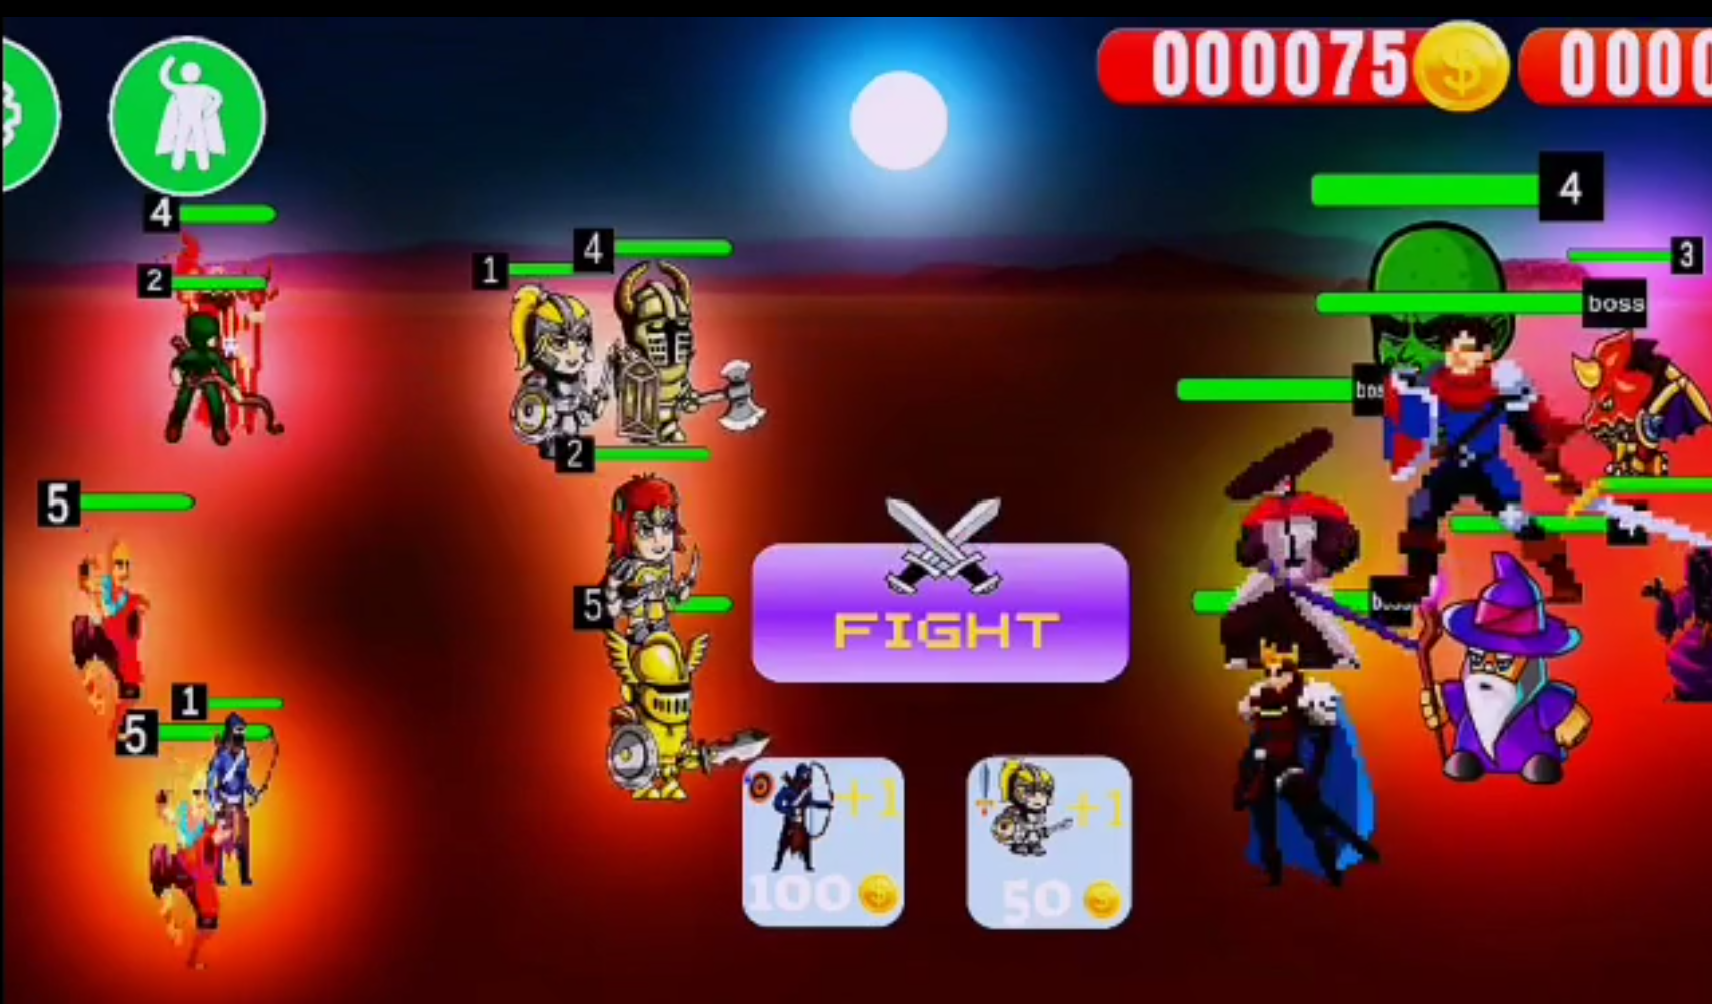
\includegraphics[width=\textwidth]{Images/AGameSuck.png}
		\vspace{0.5cm}
		\caption{Một màn chơi của game gặp vấn đề về kỹ thuật}
	\end{figure}

	\item \textbf{Lên ý tưởng và phác hoạ sơ bộ cấu trúc.}\\
	\hspace*{0.5cm}  Ở giai đoạn này, các thành viên khác trong dự án sẽ tiến hành lên ý tưởng và phác hoạ lên diẽn biến chính của cốt truyện cũng như xác định sơ bộ các thành phần khác của trò chơi như hình ảnh, âm thanh. Để việc thiết kế được dễ dàng hơn, người thiết kế có thể chia màn chơi thành các zone nhỏ sao cho dễ quản lý. Người thiết kế nên nghĩ đến màn chơi nếu chia thành nhiều zone sẽ ra sao và thiết kế từng zone riêng biệt để đạt hiệu suất cao và đơn giản hơn so với thiết kế toàn bộ màn chơi là một khối lớn.\\ 
	
	
	\item \textbf{Vẽ Bubble Diagram (lưu đồ Bong bóng).}\\
	\hspace*{0.5cm}  Trước khi bắt đầu đầu tư vào dự án, cần phải biết được tổng quan của các màn chơi sẽ như thế nào. việc giải thích bằng văn nếu không có sự hiệu quả sẽ gây khó hiểu cho người tiếp cận. Vì thế nên việc sử dụng lưu đồ sẽ phát huy tính hiệu quả, giúp cho người tiếp cận có cái nhìn tổng quan về màn chơi, bao gồm các zone chứa những gì và các zone được liên kết như thế nào. Ở giai đoạn này, sau khi phân chia màn chơi thành các vùng nhỏ và thiết kế chúng, người thiết kế sẽ kết nối các vùng đó với nhau thông qua một lưu đồ bong bóng.\\
	\textbf{Một số quy tắc khi vẽ lưu đồ:}
	\begin{itemize}
		\item Mỗi node trong đồ thị sẽ tượng trưng cho một zone của màn chơi.
		\item Mỗi node có thể kết nối với node khác bằng một và chỉ một mũi tên, đi từ ra từ node này đến node được chỉ định, một node có thể có thể có nhiều mũi tên chỉ ra, cũng như cũng có thể được nhiều mũi tên chỉ vào.
		\item Trên  mỗi mũi tên có thể có một ghi chú, có thể là điều kiện, ghi chú đường tắt,...
	\end{itemize}
	\begin{figure}[H]
		\centering
		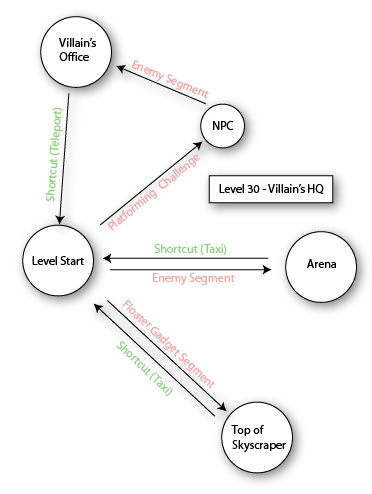
\includegraphics[width=7cm]{Images/bubblediagram.jpg}
		\vspace{0.5cm}
		\caption{Lưu đồ bong bóng}
	\end{figure}
	\hspace*{0.5cm} 
	\item \textbf{Tạo ra bản sơ lược của màn chơi}\\
	\hspace*{0.5cm}  Ở giai đoạn này, những nhà thiết kế màn chơi sẽ bắt đầu thiết kế một bản sơ lược cho màn chơi. Các bản thiết kế này có thể là thiết kế ở trên giấy, các phần mềm đồ hoạ như Adobe Illustrator hay
	trực tiếp trên các game engine như Unity, Unreal, ... Với mỗi node trong đồ thị tương ứng với một zone, một room, ta sẽ sắp xếp thứ mà người chơi sẽ phải gặp trong zone đó, đó có thể là quái vật, rương thưởng, hoặc quái vật giả rương thưởng, hoặc các câu đố đòi hỏi người chơi phải giải quyết được mới được tính là clear.  Ngoài ra, họ sẽ nghĩ đến phương pháp để kết nối các zone với nhau dựa theo mũi tên của đồ thị bong bóng cũng như điều kiện trên đó (nếu có).\\
	\hspace*{0.5cm} Để một màn chơi tổng thể hấp dẫn, dựa theo nhiều trò chơi khác đã thành công trên thị trường, mỗi zone liên tiếp nhau nên có độ khó tăng dần lên. Việc việc mỗi zone tăng dần độ khó như vậy sẽ luôn tạo cho người chơi các thách thức để họ vượt qua. Từ đó, trò chơi sẽ gia tăng trải nghiệm chơi game của người chơi.\\
	\hspace*{0.5cm} Nếu muốn di chuyển sang vùng kế tiếp thì phải clear vùng hiện tại. Ví dụ, phải clear được vùng 1 thì mới có thể đi đến vùng 2.  Vùng cuối cùng (hoặc điểm cuối cùng trên lưu đồ) sẽ là nơi được đặt một con quái vật boss hoặc mini-boss, nếu clear được thì sẽ được phần thưởng của màn chơi đó.\\
	\hspace*{0.5cm} Trong giai đoạn này, một vài thông số của màn chơi như diện tích, chiều cao, khoảng cách có thể chưa cố định. Người thiết kế và các lập trình viên sẽ kiểm thử và căn chỉnh dần cho phù hợp với ý đồ của nhà thiết kế.\\
	\item \textbf{Hoàn thành thiết kế màn chơi}\\
	\hspace*{0.5cm} Đây là giai đoạn cuối cùng, người thiết kế màn chơi sẽ hoàn thành màn chơi từ thiết kế sơ bộ ở giai đoạn 4.\\
	\hspace*{0.5cm} Người thiết kế màn chơi sẽ kết nối các vùng của màn chơi với nhau. Ở những vùng có thể di chuyển qua lại với nhau, đó có thể đơn giản chỉ là một cánh cổng hay đường hầm. Ở MeowSQL Knight, việc di chuyển 2 vùng khác nhau là tự nhiên, tuy nhiên để di chuyển cần phải clear zone hiện tại.\\
	\hspace*{0.5cm} Các zone phải được liên kết mới nhau sao cho phải với mỗi node có ít nhất một đường đi từ node bắt đầu, đi qua node hiện tại và đến node kết thúc. Nghĩa là không được có đường cùng trong màn chơi.\\
	\hspace*{0.5cm} Sau khi hoàn thành thiết lập toàn bộ bản đồ và kiểm thử, các thông số có thể thay đổi được ở giai đoạn 4 phải được thiết lập cố định lại.
\end{enumerate}
\subsubsection{Một số mẹo khi thiết kế màn chơi}
\hspace*{0.5cm}  Khi thiết kế một màn chơi, có một số mẹo chúng ta có thể tham khảo để kết quả đạt được tốt hơn.
\begin{itemize}
	\item \textbf{Thiết kế có mục đích rõ ràng: } Mỗi màn chơi phải có một mục đích tại sao nó lại tồn tại. Nó có thể là để người chơi học tập cách sử dụng một cơ chế nào đó của trò chơi và luyện tập các cơ chế đã học hoặc giúp cho cốt truyện được làm rõ và đưa đến người chơi. Ở một số trò chơi có cốt truyện, một vài màn chơi có đóng vai trò mở rộng cốt truyện ra.\\
	Từ các mục đích ban đầu, người thiết kế màn chơi phải luôn tập trung thiết kế để phục vụ mục đích đó. Tránh tập trung vào quá nhiều mục tiêu rời rạc, tránh làm level bị nhồi nhét quá nhiều. Điều này sẽ làm người chơi không bị choáng ngợp vì có quá nhiều thứ diễn ra trong màn chơi. Nếu vẫn muốn màn chơi có nhiều mục đích, hãy chắc chắn nó hợp với nhau và không làm cho màn chơi bị rối
	\item \textbf{Tập trung vào tính thực tế và sự đắm chìm khi chơi: } Tính thực tế cũng rất quan trọng và không nên xem nhẹ. Dù bối cảnh có là thế nào, viễn tưởng hoặc huyền ảo thế nào cũng nên thiết kế màn chơi sao cho người chơi cảm thấy vẫn có tính thực tế trong đó. Điển hình là trọng lực, dù cho nhân vật ở trong bất cứ thế giới game nào, thì cũng luôn bị trọng lực tác động vào. Ở các trò chơi bắn súng, người chơi thường thích việc nhà phát hành làm nó trông thực tế nhất có thể, bao gồm trọng lượng súng ảnh hưởng đến tốc độ di chuyển và độ giật khi bắn, độ giật của súng khác nhau, cũng như độ rơi của đạn khi bắn tầm xa. Trong các game về bóng đá, người chơi sẽ quan tâm đến logic trái bóng và cầu thủ trong các tình huống, về việc bắt lỗi và thẻ phạt của trọng tài, đặc biệt là các tình huống nguy hiểm trong vòng cấm.\\
	Nếu áp dụng các yếu tố thực tế một cách hợp lý, người chơi cảm nhận được sự thực tế trong trò chơi. Dần dần, họ bắt đầu chìm đắm vào trò chơi. Việc đắm chìm vô cùng quan trọng, nó cho thấy xu hướng yêu thích và sẽ gắn bó với nó lâu dài. Khi người chơi đã bắt đầu chìm đắm trong trò chơi, họ sẽ bắt đầu quan tâm đến các khía cạnh khác của trò chơi như cốt truyện, đồ hoạ, âm thanh,...
	\item \textbf{Một thử thách không quá dễ dàng nhưng không khó chịu: } Một màn chơi mang tính thử thách hoàn toàn khác với màn chơi khó đến mức gây khó chịu.\\
	Người chơi thích chơi game bởi vì tính thử thách của nó. Các thử thách này sẽ gây khó dễ cho người chơi, đòi hỏi sự rèn luyện, cùng với một khao khát mãnh liệt để vượt qua. Khi đã vượt qua được thử thách, một lượng dopamine được sinh ra khiến người chơi có cảm giác sảng khoái, khiến họ muốn tiếp tục vượt qua thử thách kế tiếp. Đây chính là mục đích cuối cùng mà các màn chơi muốn mang đến cho người chơi. Với dạng trò chơi mang tính chiến thuật như các game bóng đá, đôi khi trò chơi sẽ có một vài màn chơi khó, việc sử dụng một đội hình cố định có thể gặp khó khăn, đòi hỏi phải thay đổi chiến thuật như sử dụng cầu thủ khác, đổi sơ đồ đội hình sao cho qua được màn chơi. Người chơi sẽ cần thử nhiều loại đội hình. Đến một lúc nào đó, họ sẽ tìm ra một đội hình để vượt qua được màn chơi.\\
	Tuy nhiên, đôi khi những người thiết kế màn chơi không tránh khỏi việc trở thành một màn chơi gây khó chịu. Người thiết kế màn chơi đôi khi suy nghĩ rằng chỉ cần đưa hết tất cả những thứ khó nhất vào màn chơi sẽ làm màn chơi mang tính thách thức, hoặc họ nghĩ rằng họ có thể "bào tiền" từ người chơi thông qua các vật phẩm mua bằng tiền thật có thể giúp người chơi qua màn. Nhưng cách này có thể sẽ phản tác dụng. Nhiều trò chơi đã làm theo hướng này và gặp phải tình trạng tỉ lệ User Retention (tỉ lệ người chơi chơi tiếp) giảm đáng kể. Họ tăng độ khó các màn chơi lên rất nhiều, khiến cho việc một người chơi rèn luyện thông thường trong rất lâu để vượt qua nó trở nên bất công so với người chơi chỉ cần bỏ tiền thật để mua một vật phẩm trong cửa hàng, họ có thể dễ dàng vượt qua nó. Đây là một trong những cách làm tồi tệ, có thể giết chết tựa game của mình.\\
	Lấy ví dụ điển hình như trò chơi \textbf{Plants vs. Zombies 2}. Do là trò chơi miễn phí nên lợi nhuận thu được từ các vật phẩm trong game. Ở các phần đầu tiên sẽ xoay quanh việc người chơi xây dựng đội hình tối ưu, học các khả năng của cây mới để tiêu diệt các loại zombies mới, cũng như đi sâu trong chế độ endless mode đầy thử thách. Nếu biết tận dụng cây tốt có thể vượt qua dễ dàng. Trò chơi đón nhận được tình cảm rất lớn từ người chơi. Nhưng sang đến phần 2, nó là một nỗi thất vọng, rồi phần 3 là một thất bại ê chề, khiến cho phần game phải tái phát hành nhiều lần. Điểm mới đầu tiên là một số cây phải mua bằng tiền thật mới được mở khoá và sử dụng, khiến độ khó tăng lên nhưng nếu người chơi vận dụng tốt thì vẫn có thể phá đảo toàn bộ game. Các phiên bản về sau, nhà phát triển thêm vào hệ thống cấp độ cho cây và người chơi cần nâng cấp chúng. Càng về sau, các loại cây ban đầu gần như vô cùng yếu dù có nâng cấp và trở nên vô dụng. Người chơi gập muôn vàn khó khăn để vượt qua màn chơi. Hơn nữa, số lượng cây trả phí ngày càng nhiều lên. Chỉ cần bỏ tiền ra mua cây hoặc mua gói nâng cấp cho các cây cũ là có thể qua được dễ dàng. Điều này làm mất đi tính chiến thuật của trò chơi, khi một màn khó trong các phiên bản cũ thì chỉ cần sử dụng các cây có cấp độ cao thì qua rất dễ dàng, cộng thêm việc không có thêm các bản đồ mới làm người chơi cũng bắt đầu chán ghét và trò chơi trở nên lụi tàn. Trong những năm gần đây, các bản mod của phần 1 do fan tự làm lại được lòng rất nhiều người chơi, do tính thử thách tăng cao, đi kèm với những loại cây mới phù hợp để người chơi vượt qua thử thách.\\
	Một màn chơi không quá khó cũng không nên quá dễ, nó như vẽ đường cho hươu chạy, sẽ khiến người chơi dễ chán nản. Một màn chơi cũng không nên có quá nhiều hướng dẫn chơi hiện lên, việc hiện hướng dẫn chơi cho người chơi đi đúng hướng là tốt, nhưng có quá nhiều lại trở thành vấn đề khi thiết kế màn chơi, người thiết kế có thể để một số chi tiết cho người chơi tự khám phá, khi đó người chơi sẽ cảm thấy thoả mãn vì bản thân đã học được một thứ mới và đã có thể dùng những gì mới học vượt qua thử thách, mang lại sự thoả mãn. Nhìn chung, việc điều chỉnh độ khó màn chơi sẽ phụ thuộc vào đối tượng mà game đang nhắm đến.\\ 
\end{itemize}


\subsection{Thiết kế Database}
\subsubsection{Dữ liệu, thông tin}
\hspace*{0.5cm} Dữ liệu là mô tả cơ bản về sự vật, sự kiện, hoạt động và giao dịch được ghi lại, được phân loại, lưu trữ nhưng không được tổ chức để truyền đạt bất kỳ ý nghĩa cụ thể nào.\\
\hspace*{0.5cm} Những dữ liệu này cần phải được xử lý mới có thể truyền đạt dưới dạng thông tin mà mọi người có thể đọc và hiểu được. Dữ liệu đã được sắp xếp sao cho chúng có ý nghĩa và giá trị đối với người tiếp nhận. Người này sẽ diễn giải ý nghĩa và rút ra kết luận và hàm ý từ thông tin đã được cung cấp. \\
\hspace*{0.5cm} Nói cách khác, Thông tin là dữ liệu đã được xử lý, sắp xếp và mang bản chất được hướng đến một mục đích nào đó.
\subsubsection{Cơ sở dữ liệu (Database)}
\hspace*{0.5cm} Cơ sở dữ liệu (database) là một tập hợp các dữ liệu liên quan có ý nghĩa ngầm định. Các tính chất được quy định ngầm sẵn mà cơ sở dữ liệu có sẽ là: 
\begin{itemize}
	\item Cơ sở dữ liệu đại diện cho một khía cạnh nào đó của thế giới thực, được gọi là thế giới thu nhỏ hoặc vũ trụ diễn ngôn (universe of discourse - UoD). Mọi sự thay đổi trong thế giới thu nhỏ này đề được ánh xạ lên Cơ sở dữ liệu.
	\item Cơ sở dữ liệu là tập hợp dữ liệu có tính logic chặt chẽ với một số ý nghĩa vốn có. Một tập hợp dữ liệu ngẫu nhiên không thể được gọi chính xác là cơ sở dữ liệu.
	\item Cơ sở dữ liệu được thiết kế, xây dựng và lấp đầy các dữ liệu cho một mục đích cụ thể. Nó có một nhóm người dùng dự định và một số ứng dụng được hình thành trước mà những người dùng này quan tâm.
	\item Cơ sở dữ liệu có thể có nhiều kích thước và độ phức tạp khác nhau.
\end{itemize}
\subsubsection{Mô hình dữ liệu}
\hspace*{0.5cm} Theo nghĩa thông thường, mô hình dữ liệu là một loại dữ liệu trừu tượng được sử dụng để cung cấp biểu diễn ý niệm này.\\
\hspace*{0.5cm} Mô hình dữ liệu sử dụng các khái niệm logic, chẳng hạn như các đối tượng, thuộc tính của chúng và mối quan hệ giữa chúng, có thể dễ hiểu hơn đối với hầu hết người dùng so với các khái niệm lưu trữ máy tính.\\
\hspace*{0.5cm} Mô hình dữ liệu ẩn các chi tiết lưu trữ và hiện thực mà hầu hết người dùng cơ sở dữ liệu không quan tâm.\\
\hspace*{0.5cm} Mô hình dữ liệu là sự kết hợp của các thành phần sau:
\begin{enumerate}
	\item Một tập hợp các \textbf{kiểu cấu trúc dữ liệu} (các khối xây dựng của bất kỳ cơ sở dữ liệu nào tuân thủ theo mô hình)
	\item Một tập hợp các \textbf{toán tử hoặc quy tắc suy luận}, có thể được áp dụng cho bất kỳ trường hợp hợp lệ nào của các kiểu dữ liệu được liệt kê trong (1), để truy xuất hoặc lấy dữ liệu từ bất kỳ phần nào của các cấu trúc đó theo bất kỳ kết hợp nào mong muốn
	\item Một tập hợp các \textbf{quy tắc toàn vẹn chung}, ngầm định hoặc rõ ràng xác định tập hợp các trạng thái cơ sở dữ liệu nhất quán hoặc các thay đổi trạng thái hoặc cả hai. Các quy tắc này đôi khi có thể được thể hiện dưới dạng các quy tắc chèn-cập nhật-xóa.
\end{enumerate}
\hspace*{0.5cm} Một tập hợp các khái niệm có thể được sử dụng để mô tả cấu trúc của cơ sở dữ liệu. Trong đó, các kiểu dữ liệu, mối quan hệ và ràng buộc cần có đối với dữ liệu. Một tập hợp các operations cơ bản để chỉ định việc truy xuất và cập nhật trên cơ sở dữ liệu. Ta chỉ cung cấp những thứ cần thiết để đạt được một số mức độ trừu tượng bằng cách ẩn các chi tiết của data storage mà hầu hết người dùng cơ sở dữ liệu không cần.\\
\hspace*{0.5cm} Mục đích của mô hình dữ liệu có rất nhiều. Nó là công cụ để chỉ định các loại dữ liệu và tổ chức dữ liệu được phép trong một cơ sở dữ liệu cụ thể. Là cơ sở để phát triển phương pháp thiết kế chung cho cơ sở dữ liệu. Là cơ sở để đối phó với sự phát triển của cơ sở dữ liệu để có tác động logic tối thiểu đến các chương trình ứng dụng và hoạt động đầu cuối hiện có. Là cơ sở để phát triển các họ ngôn ngữ cấp rất cao để truy vấn và thao tác dữ liệu. Là trọng tâm cho kiến trúc DBMS. Và là phương tiện để nghiên cứu về các thuộc tính hành vi của các tổ chức dữ liệu thay thế.\\
\hspace*{0.5cm} Có nhiều loại mô hình dữ liệu
\begin{itemize}
	\item \textbf{Mô hình dữ liệu ý niệm (mức độ cao) - Conceptual/High-level Data Model}: Cung cấp các ý niệm gần gũi, dễ tiếp cận với dữ liệu với rất nhiều người dùng. Một trong những mô hình tiêu biểu cho loại mô hình dữ liệu này là Mô hình Thực Thể - Quan Hệ (Entity - Relationship Model)
	\item \textbf{Mô hình dữ liệu biểu diễn hoặc hiện thực - Representational/Implementation Data Models}:  Cung cấp các ý niệm mà người dùng cuối có thể hiểu nhưng không quá xa lạ với cách dữ liệu được tổ chức trong máy tính. Khác với mô hình dữ liệu ý niệm, mô hình dữ liệu này có các cấu trúc tương đồng hoặc gần giống với cấu trúc dữ liệu tổ chức trong storage, chỉ có điều người dùng cuối vẫn có thể đọc và hiểu được. Mô hình ẩn một số chi tiết về lưu trữ dữ liệu có thể được hiện trên hệ thống máy tính theo cách trực tiếp, giúp người tiếp xúc có thể hiểu được dễ dàng mà không bị rối. Tiêu biểu cho loại mô hình này là mô hình dữ liệu quan hệ hoặc mô hình dữ liệu hướng đối tượng,...
	\item \textbf{Mô hình dữ liệu vật lý (mức độ thấp) - Low-level/physical Data Model}: Cung cấp các ý niệm mô tả chi tiết về cách dữ liệu được lưu trữ
	trong máy tính.
\end{itemize}
\subsubsection{Hệ cơ sở dữ liệu và Hệ quản trị cơ sở dữ liệu}
\hspace*{0.5cm} Hệ quản trị cơ sở dữ liệu (Database Management System - DBMS) là tập hợp các công cụ phần mềm cho phép người chơi có thể tạo và duy trì cơ sở dữ liệu. Là một hệ thống phần mềm đa năng giúp tạo điều kiện thuận lợi cho các quá trình xác định, xây dựng, thao tác và chia sẻ cơ sở dữ liệu giữa nhiều người dùng và ứng dụng khác nhau.\\
\hspace*{0.5cm} Có nhiều loại Hệ quản trị cơ sở dữ liệu khác nhau được hình thành trong suốt chiều dài lịch sử, đáp ứng nhu cầu của các người dùng khác nhau. Khởi đầu với DBMS định hướng. Sau đó đến với các Hệ quản trị cơ sở dữ liệu sử dụng mô hình quan hệ làm mô hình dữ liệu, và SQL làm ngôn ngữ truy vấn. Về sau có các Hệ quản trị sử dụng mô hình hướng đối tượng như PostgreSQL, cũng như các hệ quản trị không sử dụng SQL hoặc sử dụng SQL cải tiến.\\
\hspace*{0.5cm} Hệ cơ sở dữ liệu (Database System - DBS) là sự kết hợp của 2 thành phần chính: Cơ sở dữ liệu và Hệ quản trị cơ sở dữ liệu. Cơ sở dữ liệu được hiện thực bằng các mô hình dữ liệu được thiết kế và hiện thực từ trước. Hệ quản trị cơ sở dữ liệu thực hiện quản lý cơ sở dữ liệu, đồng thời có thể cung cấp một số tính năng nhất định. Ví dụ như: Tổ chức tệp tin, Xử lý truy vấn, Xử lý transaction và điều khiển đồng thời,...\\
\hspace*{0.5cm} Có nhiều loại Hệ cơ sở dữ liệu khác nhau, được phân loại dựa trên nhiều yếu tố khác nhau: Phổ biến nhất là phân loại theo mô hình dữ liệu được sử dụng, loại dữ liệu, lưu trữ và tổ chức dữ liệu, kiến trúc và số lượng người dùng sử dụng đồng thời tại cùng một thời điểm.
\subsubsection{Kiến trúc Ba lớp Schema}
\begin{figure}[H]
	\centering
	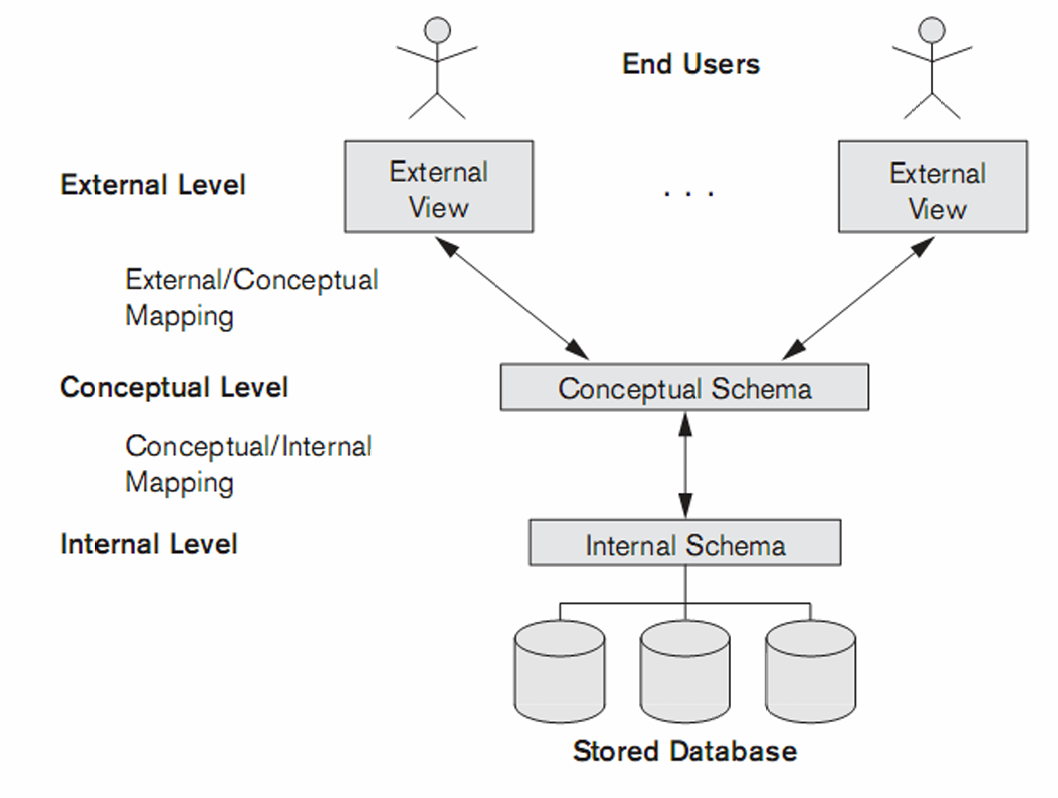
\includegraphics[width=\textwidth]{Images/ThreeSchema.png}
	\vspace{0.25cm}
	\caption{Sơ đồ biểu diễn cấu trúc 3 lớp Schema}
	\hspace*{0.5cm} Kiến trúc 3 lớp Schema bao gồm 3 thành phần là 3 lớp schema.
	\begin{enumerate}
		\item \textbf{Schema trong} mô tả cấu trúc lưu trữ vật lý của cơ sở dữ liệu
		\item \textbf{Schema luận lý} là mô tả mức độ cao của toàn bộ cơ sở dữ liệu
		\item \textbf{Schema ngoài} mô tả góc nhìn vào cơ sở dữ liệu của các nhóm người dùng khác nhau 
	\end{enumerate}
	\hspace*{0.5cm} Độc lập dữ liệu là khả năng thay đổi lược đồ ở một cấp độ của hệ thống cơ sở dữ liệu mà không cần phải thay đổi lược đồ ở cấp độ cao hơn tiếp theo.
	\begin{itemize}
		\item Độc lập dữ liệu \textbf{Luận lý}: khả năng thay đổi schema ý niệm mà không cần phải thay đổi ý niệm ngoài hoặc chương trình ứng dụng.
		\item Độc lập dữ liệu \textbf{Vật lý}: khả năng thay đổi schema trong mà không cần phải thay đổi schema ý niệm.
	\end{itemize}
\end{figure}
\subsubsection{Thiết kế Cơ sở dữ liệu}
\hspace*{0.5cm} Thiết kế Cơ sở dữ liệu là hoạt động thiết kế các cấu trúc logic và vật lý của một hoặc nhiều cơ sở dữ liệu để đáp ứng nhu cầu thông tin của người dùng trong một tổ chức cho một tập hợp các ứng dụng được xác định. Hoạt động thiết kế cơ sở dữ liệu tổng thể phải trải qua một quy trình chung có hệ thống được gọi là phương pháp thiết kế, cho dù cơ sở dữ liệu mục tiêu được quản lý bởi Hệ quản trị Cơ sở dữ liệu quan hệ hay Hệ quản trị cơ sở dữ liệu hướng đối tượng,... Kết quả của quá trình là một lược đồ cơ sở dữ liệu được định nghĩa cố định và khó có thể sửa sau khi cơ sở dữ liệu được hiện thực.\\
\hspace*{0.5cm} Mục tiêu cần đạt được trong việc thiết kế cơ sở dữ liệu tập trung chủ yếu vào việc đáp ứng các yêu cầu về nội dung thông tin của người dùng và ứng dụng được chỉ định. Cung cấp cấu trúc thông tin tự nhiên và dễ hiểu. Cũng như hỗ trợ các yêu cầu xử lý và bất kỳ mục tiêu hiệu suất nào, chẳng hạn như thời gian phản hồi, thời gian xử lý và không gian lưu trữ.\\
\begin{figure}[H]
	\centering
	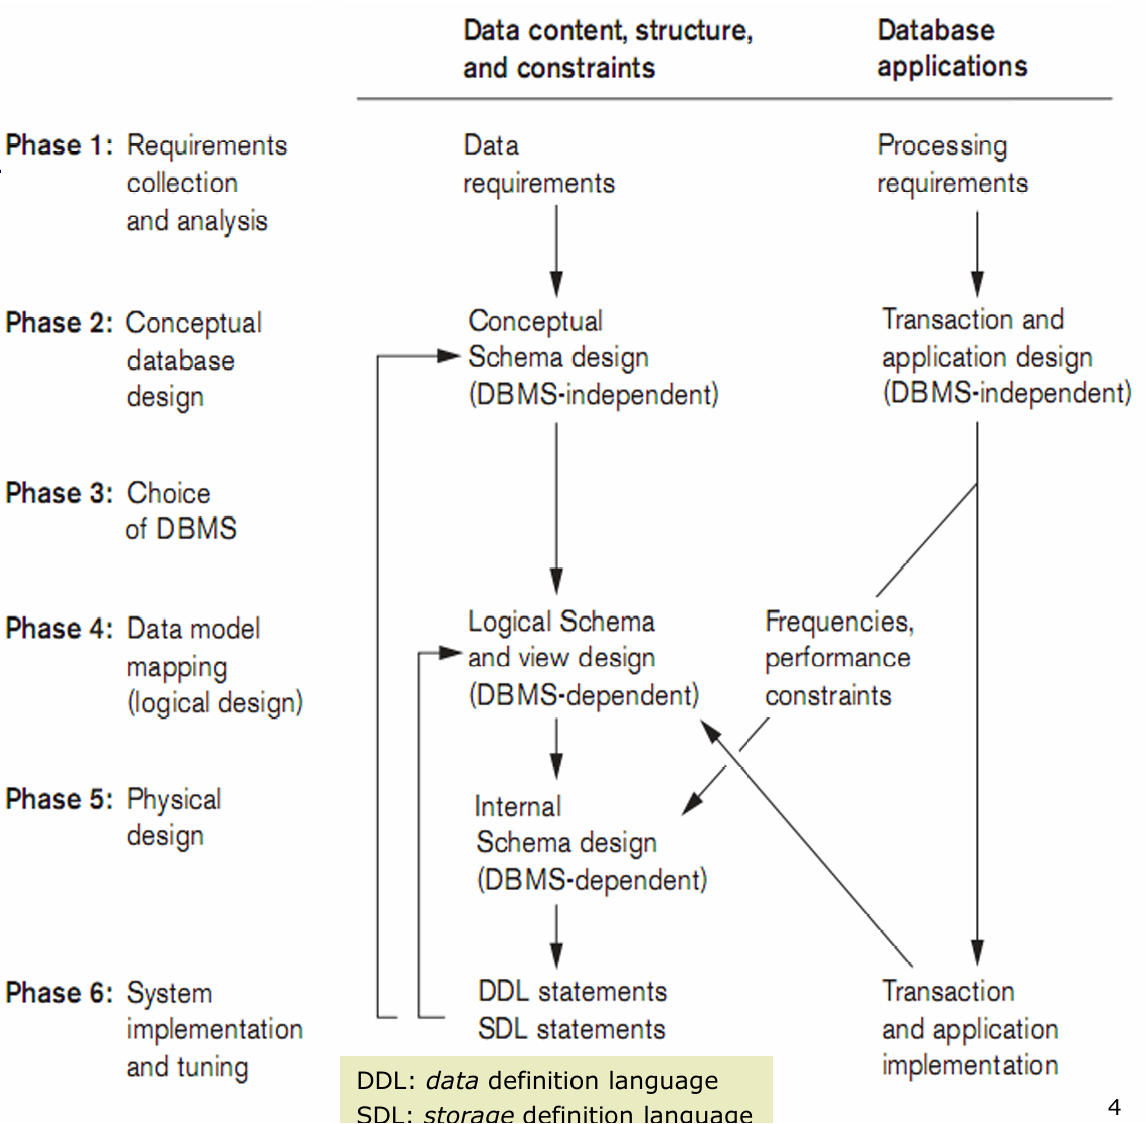
\includegraphics[width=\textwidth]{Images/DBDesign.png}
	\vspace{0.5cm}
	\caption{Quy trình thiết kế cơ sở dữ liệu}
\end{figure}
\hspace*{0.5cm} Việc thiết kế cơ sở dữ liệu trải qua 6 giai đoạn chính:
\begin{itemize}
	\item \textbf{Giai đoạn 1: Thu thập và phân tích yêu cầu}\\
	\hspace*{0.5cm} Ở bước này, người thiết kế sẽ thu thập và phân tích yêu cầu từ người dùng và ứng dụng sẽ tương tác với hệ thống cơ sở dữ liệu. Những yêu cầu này có thể được thu thập theo nhiều cách khác nhau. Trước hết cần phải xác định Lĩnh vực hoạt động chính của ứng dụng, cũng như nhóm người dùng sẽ sử dụng cơ sở dữ liệu hoặc công việc sẽ ảnh hưởng đến cơ sở dữ liệu. Tìm hiểu về tài liệu của ứng dụng sử dụng, tìm hiểm về môi trường thực thi và các kế hoạch sử dụng dữ liệu và xử lý thành thông tin, bao gồm loại giao dịch, tần suất, các yếu tố địa lý, input và output của giao dịch. Ngoài ra cần thu thập các ý kiến của người dùng về nhu cầu sử dụng, vì ưu tiên về nhu cầu của người dùng vẫn là trên hết. Quá trình này mất nhiều thời gian nhưng đóng vai trò rất quan trọng đối với sự thành công của cơ sở dữ liệu. Người thiết kế phải cố gắng xác định và phân tích kỳ vọng của người dùng và mục đích sử dụng của cơ sở dữ liệu một cách chi tiết nhất có thể để đạt được hệ cơ sở dữ liệu hiệu quả, đạt yêu cầu và giá trị mang lại cao.
	\item \textbf{Giai đoạn 2: Thiết kế cơ sở dữ liệu luận lý}\\
	\hspace*{0.5cm} Giai đoạn được chia làm 2 công việc con. Đầu tiên là thiết kế Schema Ý niệm. Mục tiêu cần đạt của công việc này là hiểu được đầy đủ về cấu trúc cơ sở dữ liệu, ngữ ngữa, mối quan hệ tương hỗ và ràng buộc. Người thiết kế cần xác định rõ được kiểu thực thể, kiểu quan hệ, thuộc tính, thuộc tính chính, số lượng và ràng buộc tham gia vào các mối quan hệ, kiểu thực thể yếu, phân cấp chuyên môn hoá/tổng quát hoá,… Người thiết kế có thể lựa chọn các cách tiếp cận yêu cầu của các ngôi để thiết kế mô hình ý niệm. Người thiết kế  có thể tổng hợp các yêu cầu lại thành một thể, rồi thiết kế ý niệm dựa trên những yêu cầu đã kết hợp đó. Hoặc cũng có thể thiết kế ý niệm cho từng nhóm yêu cầu của người dùng khác nhau, rồi tổng hợp các mô hình lại trước khi thực hiện thiết kế luận lý. Cách tiếp cận khác nhau cũng ảnh hưởng đến việc xây dựng external schema cho từng người dùng khác nhau.\\
	\hspace*{0.5cm} Một công việc trong giai đoạn này người thiết kế cần lưu tâm, đó là thiết kế giao dịch (Transaction Design), Thiết kế giao dịch bao gồm thiết kế các đặc điểm của các giao dịch (hoặc ứng dụng) cơ sở dữ liệu đã biết độc lập với DBMS để đảm bảo rằng lược đồ cơ sở dữ liệu sẽ bao gồm tất cả thông tin mà các giao dịch này yêu cầu. Xác định đầu vào/đầu ra và hành vi chức năng của giao dịch. Nhóm các giao dịch thành ba loại: giao dịch truy xuất, giao dịch cập nhật (gồm thêm dữ liệu, xoá dữ liệu và cập nhật dữ liệu), giao dịch hỗn hợp.
	\item \textbf{Giai đoạn 3: Lựa chọn Hệ quản trị cơ sở dữ liệu}\\
	\hspace*{0.5cm} Ở giai đoạn này, người thiết kế cần lựa chọn Hệ quản trị cơ sở dữ liệu phù hợp với nhu cầu của người dùng, cũng đáp ứng với điều kiện của hệ thống hiện có. Một số tác nhân có thể ảnh hưởng đến việc lựa chọn Hệ quản trị. Nó có thể là các tác nhân về kỹ thuật như tính phù hợp và loại DBMS cho tác vụ cần làm; Cấu trúc lưu trữ và đường dẫn truy cập, giao diện người dùng và lập trình viên, ngôn ngữ truy vấn cấp cao, các công cụ phát triển, tuỳ chọn kiến trúc,… được DBMS hỗ trợ; Tính di động của DBMS giữa các loại phần cứng khác nhau. Cũng có thể là các tác nhân phi kỹ thuật như chi phí mua phần mềm, chi phí bảo trì, chi phí mua phần cứng, chi phí tạo và chuyển đổi cơ sở dữ liệu, chi phí nhân sự, chi phí đào tạo, chi phí vận hành cũng như tính khả dụng của dịch vụ nhà cung cấp
	\item \textbf{Giai đoạn 4: Mapping Mô hình dữ liệu (Thiết kế cơ sở dữ liệu luận lý)}\\
	\hspace{0.5cm} Giai đoạn này các người thiết kế sẽ tạo schema ý niệm và các schema ngoài trong mô hình được hỗ trợ bởi Hệ quản trị cơ sở dữ liệu theo kiến trúc 3 schema.
	Kết quả của giai đoạn này sẽ là các câu lệnh định nghĩa dữ liệu (Data Definition Language) bằng ngôn ngữ của Hệ quản trị cơ sở dữ liệu đã chọn, chỉ định lược đồ cấp khái niệm và cấp bên ngoài của hệ thống cơ sở dữ liệu.
	\item \textbf{Giai đoạn 5: Thiết kế cơ sở dữ liệu vật lý}\\
	\hspace*{0.5cm} Giới hạn trong việc lựa chọn các cấu trúc phù hợp nhất cho
	các tệp cơ sở dữ liệu từ các tùy chọn do DBMS đó cung cấp.
	Chọn các cấu trúc lưu trữ cụ thể và đường dẫn truy cập cho
	các tệp cơ sở dữ liệu, việc lựa chọn dựa trên các yêu cầu nhất định, như thời gian phản hồi, không gian lưu trữ hiệu dụng cũng như khối lượng giao dịch. Ước tính kích thước bản ghi và số lượng bản ghi trong mỗi tệp cơ sở dữ liệu.
	Người thiết kế cần ước tính các mẫu cập nhật và truy xuất cho tệp tích lũy từ tất cả các giao dịch, cũng như ước tính sự phát triển của tệp, theo kích thước bản ghi do các thuộc tính mới hoặc theo số lượng bản ghi.
	\item \textbf{Giai đoạn 6: Hiện thực và tinh chỉnh Hệ cơ sở dữ liệu}\\
	\hspace*{0.5cm} Ở giai đoạn này, người thiết kế thực hiện các công việc như tạo các Schema cơ sở dữ liệu và các tệp tin cơ sở dữ liệu (trống); Định dạng lại dữ liệu để tải vào cơ sở dữ liệu mới nếu cần; Tải hoặc thêm dữ liệu vào bảng (nếu cần); Hiện thực các giao dịch cơ sở dữ liệu tham chiếu đến các thông số kỹ thuật ý niệm của giao dịch, sau đó viết và kiểm tra mã chương trình bằng các lệnh thuộc ngôn ngữ xử lý dữ liệu (Data Manipulation Language) nhúng. Việc điều chỉnh cơ sở dữ liệu vẫn tiếp tục miễn là cơ sở dữ liệu vẫn tồn tại, miễn là các vấn đề về hiệu suất vẫn được phát hiện và trong khi các yêu cầu vẫn thay đổi.
	
\end{itemize}
\subsection{Ngôn ngữ truy vấn SQL}
\subsubsection{SQL là gì?}
\hspace*{0.5cm} SQL được viết tắt từ Structured Query Language, là một ngôn ngữ lập trình phục vụ việc lưu trữ và xử lý thông tin trong cơ sở dữ liệu quan hệ. Cơ sở dữ liệu quan hệ lưu trữ thông tin dưới dạng bảng có các hàng và cột đại diện cho những thuộc tính dữ liệu và nhiều mối quan hệ khác nhau giữa các giá trị dữ liệu. Bạn có thể sử dụng các câu lệnh SQL để lưu trữ, cập nhật, loại bỏ, tìm kiếm và truy xuất thông tin từ cơ sở dữ liệu. Bạn cũng có thể sử dụng SQL để duy trì và tối ưu hóa hiệu suất cơ sở dữ liệu.\\
\hspace*{0.5cm} Ngôn ngữ truy vấn có cấu trúc (SQL) là một ngôn ngữ truy vấn phổ biến thường được sử dụng trong tất cả các loại ứng dụng. Các nhà phân tích và phát triển dữ liệu tìm hiểu và sử dụng SQL do ngôn ngữ này tích hợp hiệu quả với nhiều ngôn ngữ lập trình khác nhau. Theo ANSI (American National Standards Institute - Viện Tiêu chuẩn Quốc gia Hoa Kỳ), SQL là ngôn ngữ tiêu chuẩn cho các hệ thống quản lý cơ sở dữ liệu quan hệ.
\subsubsection{SQL hoạt động như thế nào?}
\hspace*{0.5cm} Việc triển khai ngôn ngữ truy vấn có cấu trúc (SQL) liên quan đến một máy chủ xử lý truy vấn cơ sở dữ liệu và trả về kết quả. Quá trình SQL đi qua một số thành phần phần mềm sau:\\
\hspace*{0.5cm}\textbf{Trình phân tích cú pháp}\\
\hspace*{0.5cm}Trình phân tích cú pháp bắt đầu bằng cách token hóa hoặc thay thế một số từ trong câu lệnh SQL bằng các ký hiệu đặc biệt. Sau đó, nó sẽ kiểm tra câu lệnh để tìm kiếm những yếu tố sau:
\begin{itemize}
	\item Tính đúng đắn: Trình phân tích cú pháp xác minh rằng câu lệnh SQL tuân theo ngữ nghĩa SQL, hay các quy tắc, đảm bảo tính đúng đắn của câu lệnh truy vấn. Ví dụ: trình phân tích cú pháp kiểm tra xem lệnh SQL có kết thúc bằng dấu chấm phẩy hay không. Nếu thiếu dấu chấm phẩy, trình phân tích cú pháp sẽ trả về lỗi.
	\item Quyền hạn: Trình phân tích cú pháp cũng xác thực rằng người dùng đang chạy truy vấn có quyền cần thiết để thao tác với dữ liệu tương ứng. Ví dụ: chỉ người dùng quản trị mới có quyền xóa dữ liệu.
\end{itemize}

% \hspace*{0.5cm}Tính đúng đắn\\
% \hspace*{0.5cm}Trình phân tích cú pháp xác minh rằng câu lệnh SQL tuân theo ngữ nghĩa SQL, hay các quy tắc, đảm bảo tính đúng đắn của câu lệnh truy vấn. Ví dụ: trình phân tích cú pháp kiểm tra xem lệnh SQL có kết thúc bằng dấu chấm phẩy hay không. Nếu thiếu dấu chấm phẩy, trình phân tích cú pháp sẽ trả về lỗi.\\

% \hspace*{0.5cm}Quyền hạn\\
% \hspace*{0.5cm}Trình phân tích cú pháp cũng xác thực rằng người dùng đang chạy truy vấn có quyền cần thiết để thao tác với dữ liệu tương ứng. Ví dụ: chỉ người dùng quản trị mới có quyền xóa dữ liệu.\\
\hspace*{0.5cm}\textbf{Công cụ quan hệ}\\
\hspace*{0.5cm}Công cụ quan hệ, hay bộ xử lý truy vấn, tạo kế hoạch truy xuất, ghi hoặc cập nhật dữ liệu tương ứng theo cách hiệu quả nhất. Ví dụ: công cụ này kiểm tra các truy vấn tương tự, sử dụng lại các phương pháp thao tác dữ liệu trước đó hoặc tạo một phương pháp mới. Công cụ quan hệ viết kế hoạch trong mã byte, một dạng biểu diễn trung cấp của câu lệnh SQL. Cơ sở dữ liệu quan hệ sử dụng mã byte để thực hiện tìm kiếm và điều chỉnh cơ sở dữ liệu một cách hiệu quả.\\
\hspace*{0.5cm}\textbf{Công cụ lưu trữ}\\
\hspace*{0.5cm}Công cụ lưu trữ, hoặc công cụ cơ sở dữ liệu, là thành phần phần mềm xử lý mã byte và chạy câu lệnh SQL dự định. Công cụ này đọc và lưu trữ dữ liệu trong các tệp cơ sở dữ liệu trên ổ đĩa lưu trữ vật lý. Sau khi hoàn tất, công cụ lưu trữ trả về kết quả cho ứng dụng yêu cầu.
\subsubsection{Các ngôn ngữ truy vấn dữ liệu SQL}
\hspace*{0.5cm}Lệnh ngôn ngữ truy vấn có cấu trúc (SQL) là những từ khóa hoặc câu lệnh SQL cụ thể được các nhà phát triển sử dụng để thao tác với dữ liệu được lưu trữ trong cơ sở dữ liệu quan hệ. Bạn có thể phân loại các lệnh SQL như sau:\\
\hspace*{0.5cm}\textbf{Ngôn ngữ định nghĩa dữ liệu}\\
\hspace*{0.5cm}Ngôn ngữ định nghĩa dữ liệu (DDL) là các lệnh SQL thiết kế cấu trúc cơ sở dữ liệu. Các kỹ sư cơ sở dữ liệu sử dụng DDL để tạo và điều chỉnh các đối tượng cơ sở dữ liệu dựa trên các yêu cầu nghiệp vụ. Ví dụ: kỹ sư cơ sở dữ liệu sử dụng lệnh CREATE để tạo các đối tượng cơ sở dữ liệu như bảng, chế độ xem và chỉ mục.\\
\hspace*{0.5cm}\textbf{Ngôn ngữ truy vấn dữ liệu}\\
\hspace*{0.5cm}Ngôn ngữ truy vấn dữ liệu (DQL) bao gồm các lệnh hướng dẫn để truy xuất dữ liệu được lưu trữ trong cơ sở dữ liệu quan hệ. Các ứng dụng phần mềm sử dụng lệnh SELECT để lọc và trả về kết quả cụ thể từ một bảng SQL.\\
\hspace*{0.5cm}\textbf{Ngôn ngữ thao tác dữ liệu}\\
\hspace*{0.5cm}Các câu lệnh ngôn ngữ thao tác dữ liệu (DML) viết thông tin mới hoặc điều chỉnh các bản ghi hiện có trong cơ sở dữ liệu quan hệ. Ví dụ: một ứng dụng sử dụng lệnh INSERT để lưu trữ một bản ghi mới trong cơ sở dữ liệu.\\
\hspace*{0.5cm}\textbf{Ngôn ngữ kiểm soát dữ liệu}\\
\hspace*{0.5cm}Quản trị viên cơ sở dữ liệu sử dụng ngôn ngữ kiểm soát dữ liệu (DCL) để quản lý hoặc cấp quyền truy cập cơ sở dữ liệu cho người dùng khác. Ví dụ: họ có thể sử dụng lệnh GRANT để cho phép các ứng dụng nhất định thao tác với một hoặc nhiều bảng.\\
\hspace*{0.5cm}\textbf{Ngôn ngữ kiểm soát giao dịch}\\
\hspace*{0.5cm}Công cụ quan hệ sử dụng ngôn ngữ kiểm soát giao dịch (TCL) để tự động thực hiện các thay đổi đối với cơ sở dữ liệu. Ví dụ: cơ sở dữ liệu sử dụng lệnh ROLLBACK để hoàn tác một giao dịch bị lỗi.
\begin{figure}[H]
	\centering
	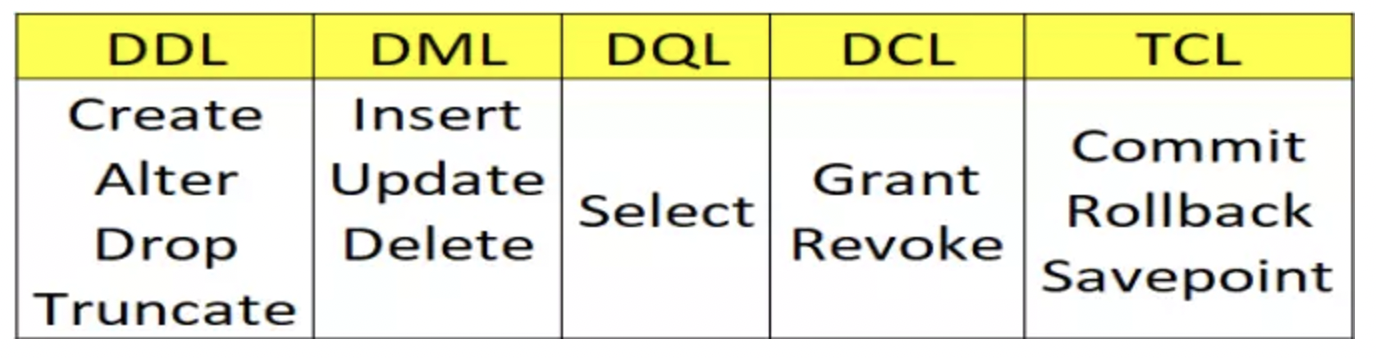
\includegraphics[width=\textwidth]{Images/lệnh SQL.png}
	\vspace{0.5cm}
	\caption{Các câu lệnh SQL cơ bản}
\end{figure}
\subsection{SQLite}
\subsubsection{SQLite là gì?}
\hspace*{.5cm}SQLite là hệ quản trị cơ sở dữ liệu (DBMS) quan hệ tương tự như Mysql,  ... Đặc điểm nổi bật của SQLite so với các DBMS khác là gọn, nhẹ, đơn giản, đặt biệt không cần mô hình Server - Client, không cần cài đặt, cấu hình hay khởi động nên không có khái niệm User, Password hay quyền hạn trong SQLite Database. Dữ liệu cũng được lưu ở một file duy nhất.\\
\hspace*{.5cm} SQLite thường không được sử dụng với các hệ thống lớn nhưng với những hệ thống ở quy mô vừa và nhỏ thì SQLite không thua các DBMS khác về chức năng hay tốc độ. Vì không cần cài đặt hay cấu hình nên SQLite được sử dụng nhiều trong việc phát triển, thử nghiệm vì tránh được những rắc rối trong quá trình cài đặt.
\subsubsection{Ưu điểm}
\begin{itemize}
	\item Giao dịch trong SQLite tuân thủ theo nguyên tắc (ACID) ngay cả sau khi hệ thống treo và mất điện.
	\item SQLite không cần mô hình Client – Server để hoạt động. Các thao tác dữ liệu trên SQLite chạy nhanh hơn so với các hệ quản trị cơ sở dữ liệu theo mô hình Client – Server.
	\item SQLite không cần phải cấu hình. SQLite rất đơn giản và dễ dàng sử dụng.
	\item SQLite hỗ trợ hầu hết các tính năng của ngôn ngữ truy vấn SQL theo chuẩn SQL92.
	\item Một sở dữ liệu hoàn chỉnh được lưu trữ trong một tệp đa nền tảng duy nhất. Phù hợp với sử dụng dưới dạng định dạng tệp ứng dụng.
	\item Một sở dữ liệu hoàn chỉnh được lưu trữ trong một tệp đa nền tảng duy nhất. Phù hợp với sử dụng dưới dạng định dạng tệp ứng dụng.
	\item Đa nền tảng: Android, iOS, Linux, Mac, Solaris, Windows,.. Dễ dàng dịch chuyển sang các hệ thống khác.
	\item SQLite rất nhỏ gọn, bản đầy đủ các tính năng nhỏ hơn 500kb, và có thể nhỏ hơn nếu lược bớt một số tính năng. Với đặc tính nhỏ gọn, truy xuất dữ liệu nhanh SQLite thường được sử dụng để nhúng vào các dự án.
\end{itemize}
\subsubsection{Nhược điểm}
\begin{itemize}
	\item Một số tính năng của SQL92 không được hỗ trợ trong SQLite như ALTER DROP COLUMN, ADD CONSTRAINT, RIGHT JOIN, TRIGGER, phân quyền GRANT và REVOKE.
	\item Vì SQLite không cần cấu hình, cài đặt, không hỗ trợ GRANT và REVOKE nên việc phân quyền truy cập cơ sở dữ liệu chỉ có thể là quyền truy cập file của hệ thống.
	\item Do sử dụng cơ chế coarse-gained locking nên trong cùng một thời điểm SQLite có thể hỗ trợ nhiều người đọc dữ liệu, nhưng chỉ có 1 người có thể ghi dữ liệu.
	\item SQLite không phải là lựa chọn hoàn hảo để đáp ứng các nhu cầu xử lý trên một khối lượng dữ liệu lớn, phát sinh liên tục.
\end{itemize}
\subsection{Dependency Injection Design Pattern} 
\subsubsection{Dependency Injection là gì?}
\hspace*{0.5cm} Dependency Injection Design Pattern là một quá trình trong đó chúng ta tiêm (inject) đối tượng phụ thuộc (dependencies) của một lớp vào một lớp phụ thuộc đối tượng đó. Dependency Injection Design Pattern là mẫu thiết kế được sử dụng phổ biến nhất hiện nay để loại bỏ sự phụ thuộc giữa các đối tượng.\\
\hspace*{0.5cm} Dependency Injection (DI) là một mẫu thiết kế được sử dụng để triển khai Inversion of Control. Nó cho phép tạo các đối tượng phụ thuộc bên ngoài một lớp và cung cấp các đối tượng đó cho một lớp phụ thuộc vào nó. Mẫu thiết kế DI bao gồm 3 lớp:
\begin{itemize}
	\item Lớp Client: Lớp Client (lớp phụ thuộc) là lớp phụ thuộc vào Lớp Service. Điều đó có nghĩa là Lớp Client muốn sử dụng các Dịch vụ (Phương thức) của Lớp Service.
	\item Lớp Service: Lớp Service (phụ thuộc) là lớp cung cấp các dịch vụ thực tế cho lớp máy khách.
	\item Lớp Injector: Lớp Injector là lớp đưa đối tượng Lớp dịch vụ vào Lớp máy khách.
\end{itemize}
\begin{figure}[H]
	\centering
	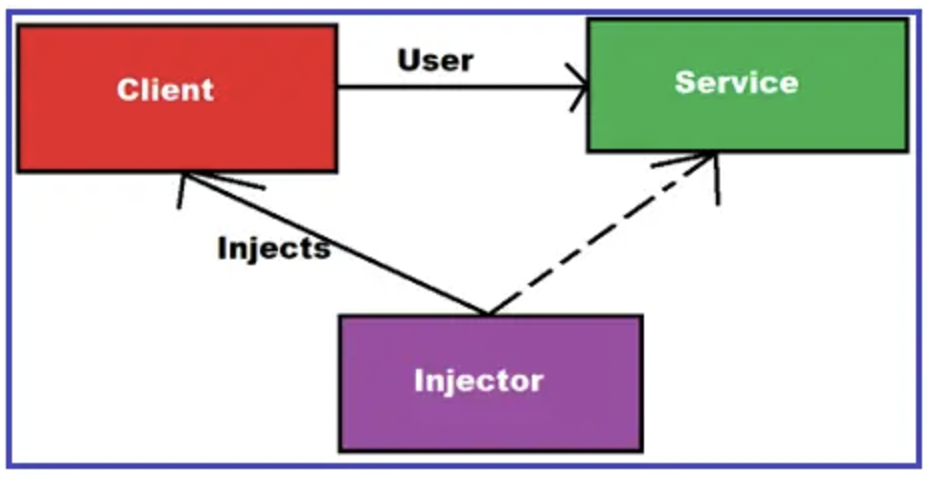
\includegraphics[width=\textwidth]{Images/DI_diagram.png}
	\vspace{0.25cm}
	\caption{Sơ đồ biểu diễn Dependency Injection}
\end{figure}
\hspace*{0.5cm} Như bạn có thể thấy, Lớp Injector tạo một đối tượng của Lớp dịch vụ và inject đối tượng đó vào Lớp Client. Sau đó, Lớp Client sử dụng Đối tượng được inject của Lớp Service để gọi các Phương thức của Lớp Service. Vì vậy, theo cách này, DI tách trách nhiệm tạo đối tượng của lớp Service ra khỏi Lớp Client. 
\subsubsection{Các loại Dependency Injection}
\hspace*{0.5cm} Lớp Injector đưa Dependency Object vào Lớp Client theo ba cách khác nhau:
\begin{itemize}
	\item Constructor injection: Các dependency (biến phụ thuộc) được cung cấp thông qua constructor (hàm tạo lớp).
	\item Setter injection: Các dependency sẽ được truyền vào 1 class thông qua các setter method (hàm setter).
	\item Interface injection: Dependency sẽ cung cấp một Interface, trong đó có chứa hàm có tên là Inject. Các client phải triển khai một Interface mà có một setter method dành cho việc nhận dependency và truyền nó vào class thông qua việc gọi hàm Inject của Interface đó.
\end{itemize}
\hspace*{0.5cm} Trong ba kiểu Inject thì phương thức Constructor injection là phổ biến nhất vì tính linh hoạt, mềm dẻo và dễ xây dựng thư viện DI.
\subsubsection{Ưu và khuyết điểm}
\hspace*{0.5cm} \textbf{Ưu điểm}
\begin{itemize}
	\item Giảm sự kết dính giữa các module.
	\item Code dễ bảo trì, dễ thay thế module.
	\item Rất dễ test và viết Unit Test.
	\item Dễ dàng thấy quan hệ giữa các module (Vì các dependency đều được inject vào constructor).
\end{itemize}
\hspace*{0.5cm} \textbf{Khuyết điểm}
\begin{itemize}
	\item Các developer mới sẽ gặp khó khăn khi học về DI.
	\item Sử dụng interface nên đôi khi sẽ khó debug, do không biết chính xác module nào được gọi.
	\item Các object được khởi tạo toàn bộ ngay từ đầu, có thể làm giảm performance.
	\item Làm tăng độ phức tạp của code.
\end{itemize}
\subsection{Observer Design Pattern}
\subsubsection{Giới thiệu}
\begin{itemize}
	\item Observer Pattern là một mẫu thiết kế thuộc nhóm Behavioral Pattern.
	\item Định nghĩa mối phụ thuộc một - nhiều giữa các đối tượng để khi mà một đối tượng (subject) có sự thay đổi trạng thái, tất cả các thành phần phụ thuộc của nó (observer) sẽ được thông báo và cập nhật một cách tự động.
	\item Một đối tượng có thể thông báo đến một số lượng không giới hạn các đối tượng khác.
\end{itemize}
\hspace*{0.5cm} Observer Pattern được áp dụng khi:
\begin{itemize}
	\item Sự thay đổi trạng thái ở 1 đối tượng có thể được thông báo đến các đối tượng khác mà không phải giữ chúng liên kết quá chặt chẽ.
	\item Cần mở rộng dự án với ít sự thay đổi nhất.
\end{itemize}
\subsubsection{Kiến trúc}
\begin{figure}[H]
	\centering
	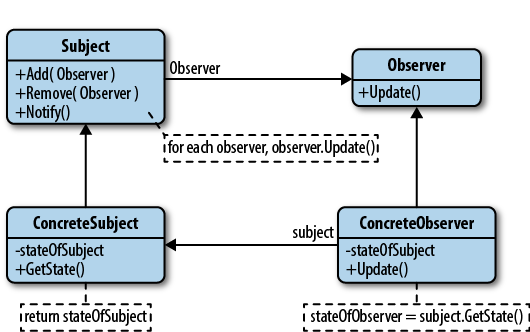
\includegraphics[width=0.75\textwidth]{Images/observer.png}
	\vspace{0.5cm}
	\caption{Kiến trúc của Observer Design Pattern}
\end{figure}
\hspace*{0.5cm} \textbf{Subject}
\begin{itemize}
	\item Biết danh sách không giới hạn các observers của nó.
	\item Cung cấp một giao diện để có thể thêm và loại bỏ observer.
\end{itemize}
\hspace*{0.5cm} \textbf{Observer}
\begin{itemize}
	\item Định nghĩa một giao diện cập nhật cho các đối tượng sẽ được subject thống báo đến khi có sự thay đổi trạng thái.
\end{itemize}
\hspace*{0.5cm} \textbf{ConcreteSubject}
\begin{itemize}
	\item Lưu trữ trạng thái danh sách các ConcreateObserver.
	\item Gửi thông báo đến các observer của nó khi có sự thay đổi trạng thái.
\end{itemize}
\hspace*{0.5cm} \textbf{ConcreteObserver}
\begin{itemize}
	\item Có thể duy trì một liên kết đến đối tượng ConcreteSubject.
	\item Lưu trữ trạng thái của subject.
	\item Thực thi việc cập nhật để giữ cho trạng thái đồng nhất với subject gửi thông báo đến.
\end{itemize}
\hspace*{0.5cm}Khi subject có sự thay đổi trạng thái, nó sẽ duyệt qua danh sách các observer của nó và gọi phương thức cập nhật trạng thái ở từng observer, có thể truyền chính nó vào phương thức để các observer có thể lấy ra trạng thái của nó và xử lý.
\begin{figure}[H]
	\centering
	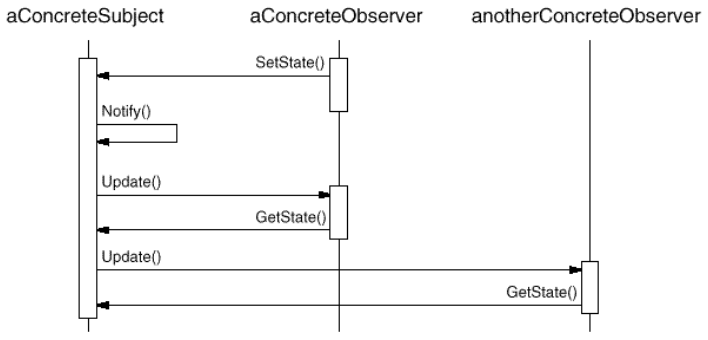
\includegraphics[width=0.75\textwidth]{Images/observer_work.png}
	\vspace{0.5cm}
	\caption{Tương tác giữa subject và các observer}
\end{figure}
\subsubsection{Ưu và nhược điểm}
\hspace*{.5cm} \textbf{Ưu điểm}
\begin{itemize}
	\item Đảm bảo nguyên tắc Open/Closed Principle (OCP): Cho phép thay đổi Subject và Observer một cách độc lập. Chúng ta có thể tái sử dụng các Subject mà không cần tái sử dụng các Observer và ngược lại. Nó cho phép thêm Observer mà không sửa đổi Subject hoặc Observer khác.
	\item Thiết lập mối quan hệ giữa các objects trong thời gian chạy.
	\item Sự thay đổi trạng thái ở 1 đối tượng có thể được thông báo đến các đối tượng khác mà không phải giữ chúng liên kết quá chặt chẽ.
	\item Không giới hạn số lượng Observer
\end{itemize}
\hspace*{.5cm} \textbf{Nhược điểm}
\begin{itemize}
	\item Unexpected update: Bởi vì các Observer không biết về sự hiện diện của nhau, nó có thể gây tốn nhiều chi phí của việc thay đổi Subject.
	\item Subscriber được thông báo theo thứ tự ngẫu nhiên.
\end{itemize}
\subsection{Unity Engine và C\#}
Trong quá trình phát triển trò chơi điện tử, mỗi một tựa game là những thực thể độc lập, được thực hiện theo những cách khác nhau và có những điểm đặc trưng riêng của tựa game đó. Tuy nhiên, việc xây dựng một tựa game từ móng thì sẽ rất tốn thời gian và công sức. Có những thành phần tổng quát, cơ bản có thể được dùng đi dùng lại cho nhiều trò chơi khác nhau. Ví dụ cách vật lý và trọng lực tác động lên các vật thể đều giống nhau. Hoặc cách phát âm thanh trong trò chơi cũng có thể tổng quát hóa được. Một ví dụ nữa là việc phát hiện và xử lý va chạm của đa số trò chơi cũng phát triển dựa trên cùng một nền tảng lý thuyết. Do đó, người ta nhận ra rằng có thể tạo ra một bộ khung (framework) hay một hệ thống (infrastructure) làm nền tảng để việc phát triển trò chơi trở nên thuận tiện và hiệu quả hơn. Bộ khung hoặc hệ thống này được gọi là game engine.\footnote{Alan Thorn, \textit{Game Engine Design and Implementation 1st Edition}, tr.6}\\

Unity là một trong những engine phát triển game phổ biến nhất hiện nay. Unity cung cấp cho người dùng một nền tảng để tạo ra các trò chơi, ứng dụng 2D và 3D một cách thuận tiện và có hệ thống. Ưu điểm của việc sử dụng engine đó là engine sẽ hỗ trợ sẵn những cơ chế cốt lõi của một trò chơi điện tử bao gồm render đồ họa 2D và 3D, tính toán vật lý và va chạm, âm thanh, animation ... Lý do nhóm nghiên cứu chọn sử dụng Unity engine bởi vì Engine này phổ biến, dễ tiếp cận và cực kỳ phù hợp với dự án game vừa và nhỏ. Một điểm cộng nữa là cộng đồng sử dụng Unity Engine rất lớn. Điều này khiến việc vừa làm vừa học hỏi trở nên dễ dàng hơn nhờ nguồn tài liệu và hướng dẫn vô cùng phong phú.\\

Ngôn ngữ lập trình được sử dụng cùng với Unity là C\#. C\# là một ngôn ngữ lập trình thuần hướng đối tượng, rất phù hợp với phát triển hệ thống component-based. Điểm mạnh của C\# là cú pháp tuy đơn giản nhưng rất chặt chẽ và linh hoạt, giúp cho nhà phát triển dễ dàng hiện thực những ý tưởng sáng tạo của mình.\\
\newpage
\section{Phân tích Thiết kế hệ thống}

\subsection{Các Stakeholder và User story}
\subsubsection{User story của Game Player}
\subsubsection{User story của Game Master}

\subsection{Các thành phần của hệ thống}

\subsection{Các yêu cầu của hệ thống}
\subsubsection{Yêu cầu chức năng}
\subsubsection{Yêu cầu phi chức năng}

\subsection{Usecase Diagram của toàn hệ thống}
\subsubsection{Usecase Diagram cho Game Client}
\subsubsection{Usecase Diagram cho Adminstrator}
\newpage
\section{Thiết kế hệ thống}
\subsection{Hệ thống xử lý câu truy vấn SQL}
\hspace*{0.5cm} Để có thể xử lý câu truy vấn được nhập từ User. Nghiên cứu các giải pháp sao cho có thể nhận câu SQL người chơi đã nhập, xử lý và trả kết quả về cho hệ thống xử lý và đưa ra các phản ứng của game. Có rất nhiều hướng tiếp cập khác nhau. Nhưng nhóm cũng lựa chọn một số hướng tiếp cận nhất định.
\subsubsection{Hướng tiếp cận sử dụng SQL Server tại Localhost}
\hspace*{0.5cm} Hướng tiếp cận này sử dụng module SQL và DB là một process độc lập và việc giao tiếp giữa DB và Game là thông qua việc kết nối Database thông qua địa chỉ Localhost và một port nhất định. Việc thiết lập SQL Database Server là riêng biệt. Về phía Game Client chỉ gần thiết lập một connector, sử dụng làm client rồi kết nối đến process Server Local. Các câu truy vấn và dữ liệu trả về sẽ được giao tiếp thông qua connector này.
\begin{figure}[H]
	\centering
	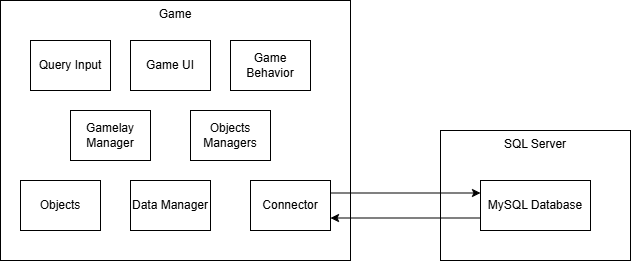
\includegraphics[width=\textwidth]{Images/SQLLocalServer.png}
	\vspace{0.5cm}
	\caption{Mô hình cấu trúc của hướng giải pháp chạy SQL Server trên Local}
\end{figure}
Dưới đây là đoạn code mẫu cho việc kết nối đến SQL Server và gọi yêu cầu thực thi truy vấn từ client\\
\begin{verbatim}
	using System;
	using MySql.Data.MySqlClient;
	
	public class DatabaseConnection
	{
		private MySqlConnection connection;
		
		public void Initialize()
		{
			string connectionString = "Server=localhost;Database=yourdatabase;Uid=yourusername;Pwd=yourpassword;";
			connection = new MySqlConnection(connectionString);
		}
		
		public void OpenConnection()
		{
			try
			{
				connection.Open();
				Console.WriteLine("Connection opened successfully.");
			}
			catch (Exception ex)
			{
				Console.WriteLine("An error occurred: " + ex.Message);
			}
		}
		
		public void CloseConnection()
		{
			try
			{
				connection.Close();
				Console.WriteLine("Connection closed successfully.");
			}
			catch (Exception ex)
			{
				Console.WriteLine("An error occurred: " + ex.Message);
			}
		}
		
		public void ExecuteQuery(string query)
		{
			try
			{
				OpenConnection();
				MySqlCommand cmd = new MySqlCommand(query, connection);
				cmd.ExecuteNonQuery();
				Console.WriteLine("Query executed successfully.");
			}
			catch (Exception ex)
			{
				Console.WriteLine("An error occurred: " + ex.Message);
			}
			finally
			{
				CloseConnection();
			}
		}
	}
\end{verbatim}
\hspace*{0.5cm} Với việc sử dụng một process riêng, ta có thể tuỳ biến process theo dạng Hệ cơ sở dữ liệu SQL nào đều được, bao gồm MySQL, PostgreSQL,... Miễn là ta lựa chọn thư viện Database Client cho Connector phù hợp là được. Ta sẽ có toàn bộ chức năng như một hệ cơ sở dữ liệu thuần tuý, ta có thể thiết lập các stored procedure, function, thiết lập các quyền cho các user khác nhau cũng như nhiều tính năng hỗ trợ hơn.\\
\hspace*{0.5cm} Tuy nhiên, với việc sử dụng một process riêng và có sử dụng port. Nếu không xử lý port hợp lý, port mà process chiếm dụng sẽ không được sử dụng cho mục đích khác nữa. Hơn nữa, việc chạy localhost server bản chất vẫn là process, và nó có thể chấm dứt bởi trình quản lý tác vụ của hệ điều hành. Nếu mất đi kết nối với server local, game sẽ không thể thực thi các tác vụ có liên quan đến SQL, game sẽ không thể hoạt động và đó là điều không thể chấp nhận được. Hơn nữa, việc khởi chạy game đòi hỏi game cũng phải khởi chạy thêm tiến trình server. Cũng như khi cài đặt trò chơi, ta phải cài đặt thêm SQL Server. Khiến cho cấu trúc lủng củng, không nhất quán, đặc biệt là nếu SQL Server có sự cố thì game cũng không hoạt động được, dẫn đến chạy không ổn định.
\subsubsection{Hướng tiếp cận xây dựng Hệ cơ sở dữ liệu SQLite ngay trong game}
\hspace*{0.5cm} Thay vì sử dụng một process riêng biệt, hướng tiếp cận này sử dụng SQLite, là một hệ cơ sở dữ liệu gọn nhẹ, có khả năng nhúng vào các ứng dụng khác. Đây là một ưu điểm lớn của SQLite khi nó có thể thực hiện các câu truy vấn ngay trong lòng ứng dụng, giúp cho cấu trúc được nhất quán và hoạt động đồng nhất và ổn định.
\begin{figure}[H]
	\centering
	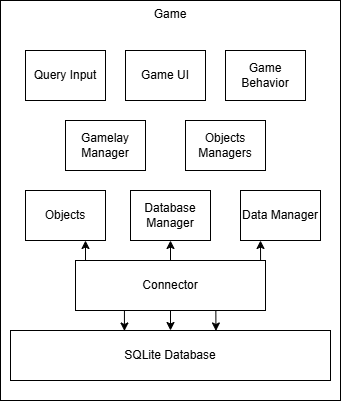
\includegraphics[width=\textwidth]{Images/SQLITE.png}
	\vspace{0.5cm}
	\caption{Cấu trúc game với Hệ cơ sở dữ liệu SQLite}
\end{figure}
\hspace{0.5cm} Cách thiết lập cũng khá đơn giản, chỉ cần một file .db, cùng với các dependencies cho SQLite hoạt động, và một module connector để kết nối với cơ sở dữ liệu cục bộ, connector cũng đóng vai trò thực hiện các câu truy vấn từ hệ thống và người chơi. Dưới đây là hai đoạn code cho Database Management va Execution cho việc kết nối database cục bộ dạng file và thực thi câu truy vấn. Đoạn code sử dụng SQliter, một công cụ hỗ trợ xử lý kết nối đễn database cục bộ.
\begin{verbatim}
	using System;
	using System.Collections;
	using System.Collections.Generic;
	using UnityEngine;
	using System.Data;
	using Mono.Data.SqliteClient;
	using System.IO;
	using System.Linq;
	using System.Text;
	using SQLiter;
	using Unity.VisualScripting.Dependencies.Sqlite;
	
	namespace Backend
	{
		public class DatabaseManagement : MonoBehaviour
		{
			public bool DebugMode = true;
			
			//public object BackendService;
			
			
			private string sqlDBLocation;
			
			
			//private const string SQL_DB_NAME = "AnimalFantasy";
			
			
			/// <summary>
			/// DB objects
			/// </summary>
			private IDbConnection connection = null;
			private IDbCommand command = null;
			private IDataReader reader = null;
			
			public IDbConnection DBConnection => new SqliteConnection(sqlDBLocation);
			public IDbCommand DBCommand => command;
			public IDataReader DBReader => reader;
			
			//private string sqlString;
			
			//public bool createNewTable = true;
			
			/// <summary>
			/// Awake will initialize the connection.  
			/// RunAsyncInit is just for show.  You can do the normal SQLiteInit to ensure that it is
			/// initialized during the AWake() phase and everything is ready during the Start() phase
			/// </summary>
			private void Awake()
			{
				//if (DebugMode)
				//	Debug.Log("--- Awake ---");
				
				// here is where we set the file location
				// ------------ IMPORTANT ---------
				// - during builds, this is located in the project root - same level as Assets/Library/obj/ProjectSettings.
				// - during runtime (Windows at least), this is located in the SAME directory as the executable.
				// you can play around with the path if you like, but build-vs-run locations need to be taken into account.
				sqlDBLocation = "URI=file:" + DBConfiguation.SQL_PATH + DBConfiguation.SQL_DB_NAME + ".db";
				
				//Debug.Log(_sqlDBLocation);
				
				//Instance = this;
				SQLiteInitialize();
				GlobalContainer.GetGameContainer.Register<DatabaseManagement>(this);
			}
			
			
			
			
			/// <summary>
			/// Clean up SQLite Connections, anything else.
			/// </summary>
			private void OnDestroy()
			{
				SQLiteClose();
			}
			
			/// <summary>
			/// Example using the Loom to run an asynchronous method on another thread so SQLite lookups.
			/// do not block the main Unity thread.
			/// </summary>
			public void RunAsyncInit()
			{
				LoomManager.Loom.QueueOnMainThread(() =>
				{
					SQLiteInitialize();
				});
			}
			
			private void SQLiteClose()
			{
				if (reader != null && !reader.IsClosed)
				reader.Close();
				reader = null;
				
				if (command != null)
				command.Dispose();
				command = null;
				
				if (connection != null && connection.State != ConnectionState.Closed)
				connection.Close();
				connection = null;
				Events.OnDBClosed.Invoke();
			}
\end{verbatim}

\begin{verbatim}
	using System;
	using System.Collections;
	using System.Collections.Generic;
	using UnityEngine;
	using System.Data;
	using Mono.Data.SqliteClient;
	using System.IO;
	using System.Linq;
	using System.Text;
	using JetBrains.Annotations;
	using SQLiter;
	using Unity.VisualScripting.Dependencies.Sqlite;
	/// <summary>
	/// Backend will be responsible for Initialize the Database, using SQL Schema as a playground where player will use SQL Language to interact with game.
	/// UserExecution will be used for processing SQL Command typed by Player, include attack() and use() procedure
	/// BackendExecution will be used for processing SQL Command demanded by the Object Manager. This will have more permission than UserExecution.
	/// Initializer (SQLInitializer) is used for Initializing the game state (include SQL State Initialize) - use to load game, level or progress.
	/// </summary>
	namespace Backend
	{
		
		public class QueryResponse
		{
			public string query;
			public bool Success;
			[CanBeNull] public List<Dictionary<string, object>> results = null;
			[CanBeNull] public Exception error = null;
		}
		
		public class QueryRequest
		{
			public CommandType CType;
			public string tableName;
			[CanBeNull] public Dictionary<string, object> data = null;
		}
		
		
		public class Execution : MonoBehaviour
		{
			
			public bool DebugMode = false;
			
			
			
			/// <summary>
			/// DB objects
			/// </summary>
			private IDbConnection _connection = null;
			private IDbCommand _command = null;
			private IDataReader _reader = null;
			
			public bool _createNewTable = true;
			
			/// <summary>
			/// Awake will initialize the connection.  
			/// RunAsyncInit is just for show.  You can do the normal SQLiteInit to ensure that it is
			/// initialized during the AWake() phase and everything is ready during the Start() phase
			/// </summary>
			void Awake()
			{
				
			
				
				GlobalContainer.GetGameContainer.Register<Execution>(this);
				
				_connection = GlobalContainer.GetGameContainer.Resolve<DatabaseManagement>().DBConnection;
				_command = _connection.CreateCommand();
			}
			
			/// <summary>
			/// Unity Start
			/// </summary>
			void Start()
			{
				
				
				// just for testing, comment/uncomment to play with it
				// note that it MUST be invoked after SQLite has initialized, 2-3 seconds later usually.  1 second is cutting it too close
			}
			
			
			
			
			/// <summary>
			/// Uncomment if you want to see the time it takes to do things
			/// </summary>
			//void Update()
			//{
				//    Debug.Log(Time.time);
				//}
			
			/// <summary>
			/// Clean up SQLite Connections, anything else
			/// </summary>
			void OnDestroy()
			{
				SQLiteClose();
			}
			
			/// <summary>
			/// Basic execute command - open, create command, execute, close
			/// </summary>
			/// <param name="commandText"></param>
			public void ExecuteNonQuery(string commandText)
			{
				_connection.Open();
				_command.CommandText = commandText;
				_command.ExecuteNonQuery();
				_connection.Close();
			}
			
			/// <summary>
			/// Clean up everything for SQLite
			/// </summary>
			private void SQLiteClose()
			{
				if (_reader != null && !_reader.IsClosed)
				_reader.Close();
				_reader = null;
				
				if (_command != null)
				_command.Dispose();
				_command = null;
				
				if (_connection != null && _connection.State != ConnectionState.Closed)
				_connection.Close();
				_connection = null;
			}
			
			public QueryResponse ExecuteQuery(string commandText)
			{
				QueryResponse result = new QueryResponse();
				try
				{
					_connection.Open();
					
					// if you have a bunch of stuff, this is going to be inefficient and a pain.  it's just for testing/show
					_command.CommandText = commandText;
					_reader = _command.ExecuteReader();
					//if (_reader.)
					
					var _header = new List<string>();
					//Debug.Log(_header);
					DataTable dt = _reader.GetSchemaTable();
					foreach (DataRow row in dt.Rows)
					{
						_header.Add(row.Field<string>("ColumnName"));
					}
					List<List<string>> rows = new List<List<string>>();
					while (_reader.Read())
					{
						// reuse same stringbuilder
						List<string> rowValue = new List<string>();
						
						for (int i = 0; i < _header.Count; i++)
						{
							rowValue.Add(_reader.GetString(i));
						}
						/*
						sb.Length = 0;
						
						sb.Append(_reader.GetString(0)).Append(" ");
						sb.Append(_reader.GetString(1)).Append(" ");
						
						sb.AppendLine();
						*/
						
						// view our output
						if (DebugMode)
						//Debug.Log(sb.ToString());
						rowValue.ToString();
						rows.Add(rowValue);
						
					}
					_reader.Close();
					_connection.Close();
					rows.Insert(0, _header);
					Events.OnSelectDisplay.Invoke(rows);
				}
				catch (Exception e)
				{
					result.Success = false;
					result.error = e;
					_reader.Close();
					_connection.Close();
					//Events.OnErrorDisplay.Invoke(e);
					//throw;
				}
				
				
				return result;
			}
		}
	}
	
\end{verbatim}
\hspace*{0.5cm} Tuy nó có sự tiện lơi và gọn nhẹ và dễ dàng nhúng vào các ứng dụng khác, nhưng đổi lại, nó phải hy sinh nhiều tính năng. Nó không hỗ trợ cấp quyền cho người dùng, nên việc xử lý trên schema sẽ phải thêm một số bước mới có thể cho kỳ vọng. Ngoài ra, với việc không có stored procedure cũng là một thiệt thòi lớn cho những ai muốn sử dụng procedure.\\
\hspace*{0.5cm} Bỏ qua những khuyết điẻm mà giải pháp này còn tồn đọng, nhóm vẫn quyết định sử dụng giải pháp này vì tính nhất quán và đồng nhất với dự án. Các vấn đề phát sinh nhóm sẽ có những cách xử lý khác nhau.
\subsection{Schema chính của game}
\hspace*{0.5cm} Một trong những thứ không thể thiếu của game là schema của trò chơi. Người chơi sẽ sử dụng các câu truy vấn SQL để khai thác tối đa SQL, tìm được mục tiêu và tiêu diệt chúng.
\begin{figure}[H]
	\centering
	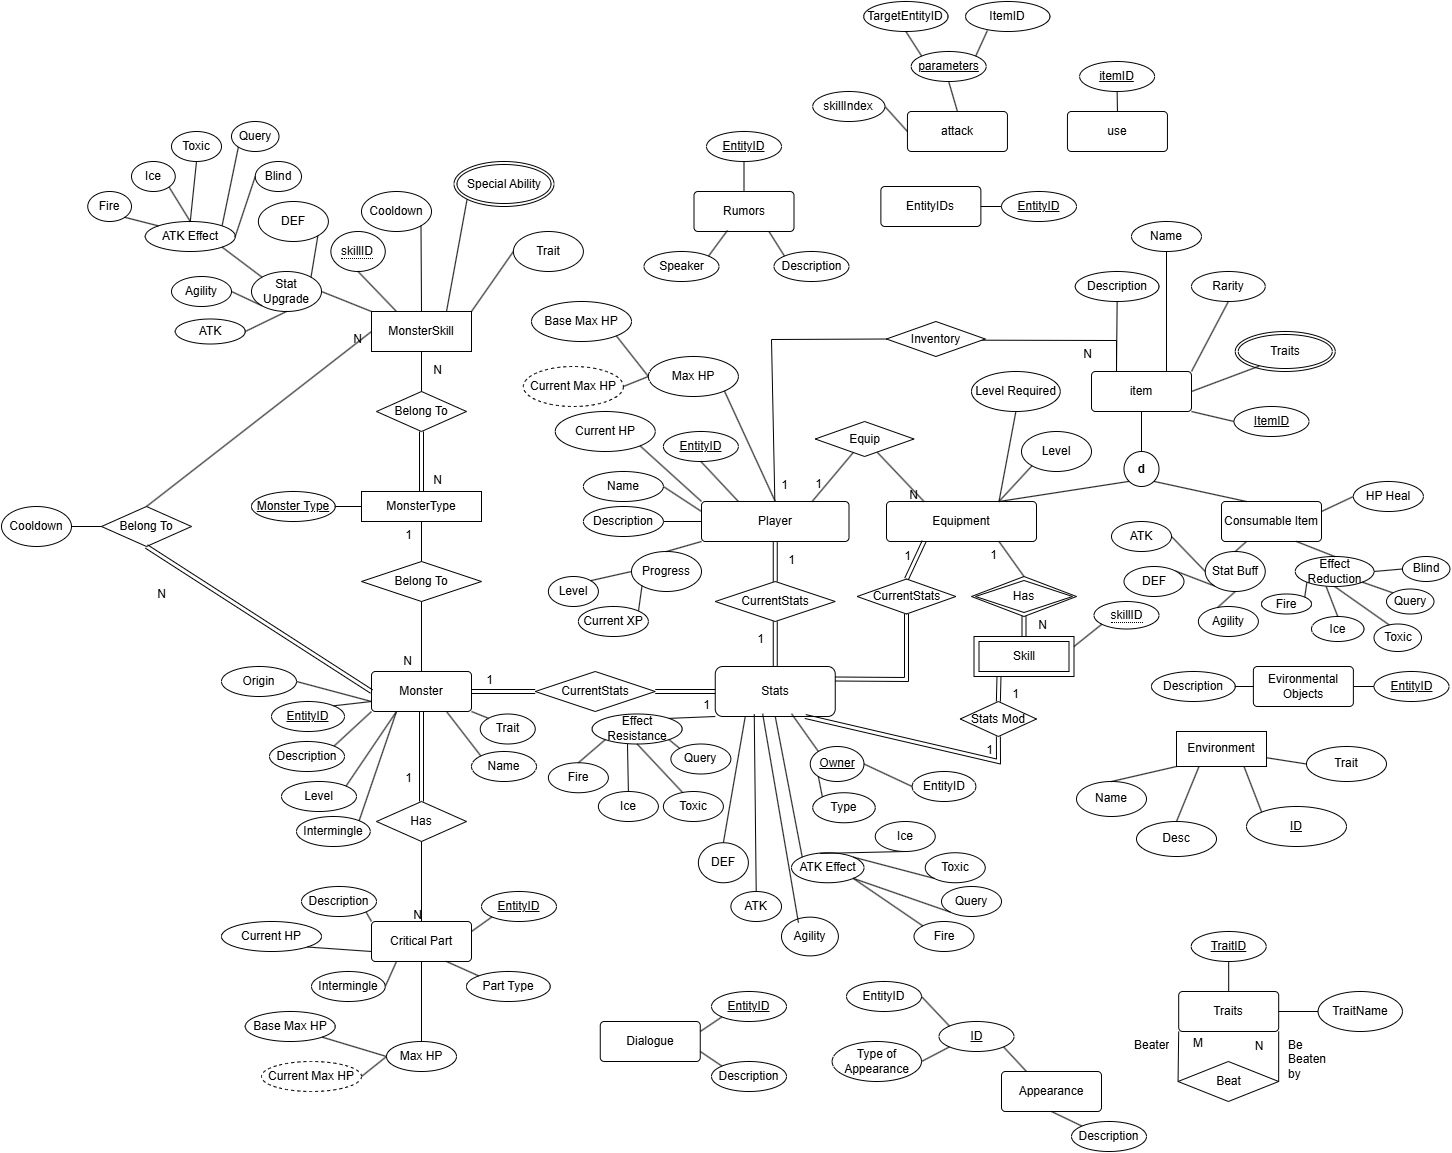
\includegraphics[width=\textwidth]{Images/SchemaEERD.png}
	\vspace{0.5cm}
	\caption{Schema EERD của game}
\end{figure}
\subsection{Xử lý các hành vi ngoại lệ của người chơi}

\hspace*{0.5cm} Trong quá trình chơi, khó mà tránh khỏi việc người chơi có những hành vi cố ý tác động đến schema, nếu không xử lý hợp lý sẽ gây tình trạng màn chơi bị rối loạn, cũng như có thể dẫn đến mất ổn định game. Luôn nhớ rằng Schema chỉ là Playground của game, các object của game chỉ được quản lý bởi hệ thống, nên việc xử lý phải mang tính răn đe, cho người chơi nhớ được mọi hành vi của bản thân đều có thể mang lại hậu quả, tương tự với việc xử lý SQL trong công việc thực tế.

\hspace*{0.5cm} Với việc nhóm quyết định sử dụng SQLite và tích hợp thẳng vào game. Khiến nó bộc lộ hạn chế lớn: nó không hỗ trợ việc phân quyền. Vì vậy nhóm quyết định đặt ra các bộ quy tắc để xử lý ở mức DB Manager khi người chơi có các hành vi sau:

\subsubsection{Chèn (Insert) dữ liệu vào các bảng}
Việc insert dữ liệu vào bảng có thể dẫn đến các hành vi phản hồi của game khác nhau:

\paragraph{Chèn vào các bảng Item, Skills}
Các Item cũng như record đã được quản lý bởi game, nên cho dù người chơi có chèn vào bao nhiêu record dữ liệu giả rồi sử dụng chúng trong hàm attack hoặc use đều vô hiệu. Schema tìm được ID trong quá trình xử lý câu lệnh nhưng đưa vào hệ thống game để thao tác mà không tìm ID cũng vô nghĩa, hệ thống sẽ thông báo đã không có gì xảy ra và lượt thao tác của người chơi kết thúc. Không như việc ID không đúng thì người chơi vẫn có cơ hội nhập lại, việc thêm ID giả vào sẽ mang lại hậu quả nghiêm trọng hơn cho người chơi.

\paragraph{Chèn vào các bảng Monster, Critical Parts}
Ngoại trừ việc chèn vào bảng để giải quyết các quái vật khó nhằn, việc chèn vào bảng các record ``rác'' là hành vi gây bất lợi cho người chơi. Vì số lượng record trong bảng lớn khiến người chơi khó xác định được record đúng (tương tự việc bộ phận quái vật tự tạo các record để ngụy trang).

\paragraph{Chèn dữ liệu vào Environment Objects}
Việc thêm dữ liệu vào Environment Objects là vô nghĩa, không mang lại lợi ích cho người chơi, mà chỉ khiến cho bảng dữ liệu to ra, gây khó khăn cho người chơi trong việc xác định entity id phù hợp.

\paragraph{Chèn record vào bảng Player}
Việc insert record của bảng player là vô nghĩa, vì sau khi insert, game sẽ update lại giá trị của player, nó bao gồm việc loại bỏ các record ``rác'' không được quản lý bởi hệ thống, việc insert là vô nghĩa.

\subsubsection{Cập nhật (Update) record của các bảng}

\paragraph{Cập nhật record của các bảng Item, Skills}
Tương tự với Insert, các Item cũng như record đã được quản lý bởi game. Cho dù người chơi có update vào bao nhiêu record dữ liệu thành theo ý của mình rồi sử dụng chúng trong hàm attack hoặc use đều không có sự thay đổi, game vẫn sẽ lấy giá trị mặc định do game đưa vào schema.

\paragraph{Cập nhật record của các bảng Monster, Critical Parts}
Ngoại trừ việc update để giải quyết các quái vật khó nhằn, việc update các record vào bảng có thể biến record đó trở thành record rác và gây bất lợi cho người chơi. Game manager không chỉ quản lý thông tin record hiện tại mà còn quản lý record trong quá khứ.

\paragraph{Cập nhật record của Environment Objects}
Việc update record của các vật thể trong môi trường có kết quả dẫn đến tương tự với việc delete. Theo gameplay, việc delete record của game object trong môi trường có thể kích hoạt hiệu ứng của vật thể đó, hiệu ứng có thể mang lại lợi thế, bất lợi, thậm chí còn mang hậu quả nghiêm trọng (ví dụ sát thương cho người chơi quá lớn, làm người chơi chết).

\paragraph{Cập nhật record của bảng Player}
Việc update record của bảng player là vô nghĩa, vì sau khi update, game sẽ khôi phục giá trị player về trước khi nó được update.

\subsubsection{Xóa (Delete) dữ liệu khỏi các bảng}

\paragraph{Xóa record các bảng Item, Skills}
Việc xoá record của bảng Item, Skills sẽ mang lại bất lợi cho người chơi. Khi người chơi thực hiện hàm attack, use thì schema sẽ báo lỗi không tìm thấy id phù hợp, khi đó người chơi đến hết màn chơi không thể sử dụng hoặc tấn công bằng item đó nữa.

\paragraph{Xóa record các bảng Monster, Critical Parts}
Ngoại trừ việc xoá record để giải quyết các vấn đề phát sinh từ quái vật khó nhằn, đây là hành vi gây bất lợi cho người chơi. Nếu mất đi record cần thiết, người chơi sẽ không thể xác định được record của bộ phận monster, việc thực thi câu lệnh attack() sẽ trả lỗi ở mức Database.

\paragraph{Xóa dữ liệu Environment Objects}
Tương tự với update record, việc delete record của game object trong môi trường có thể kích hoạt hiệu ứng của vật thể đó, hiệu ứng có thể mang lại lợi thế, bất lợi, thậm chí còn mang hậu quả nghiêm trọng.

\paragraph{Xóa record bảng Player}
Với việc bảng player tự phục hồi, nên việc delete record không có ảnh hưởng gì.



\newpage
\section{Tổng kết}
\subsection{Nhận xét}
\hspace*{1cm} Đến thời điểm hiện tại, dự án MeowSQL Knight đã gần như hoàn thiện về mặt design, một phiên bản mẫu cũng đang trong giai đoạn phát triển. Mặc dù còn tồn tại nhiều lỗi và một số tính năng chưa được phát triển đầy đủ so với thiết kế ban đầu, nhưng nó vẫn là sự nỗ lực của cả nhóm trong việc cố gắng hoàn thành đồ án của trò chơi.\\
\hspace*{1cm} Mục tiêu của nhóm là một trò chơi chiến đấu sử dụng ngôn ngữ truy vấn SQL. Với chế độ chơi đơn theo cốt truyện, nơi người chơi sẽ đi vào tầng sâu nhất của thế giới game để tìm ra bí ẩn cho những bất thường diễn ra trong thế giới game của nhân vật chính. Người chơi phải chiến đấu với các quái vật ngăn cản người chơi trên đường đi bằng các câu truy vấn SQL. Với select để tra cứu thông tin schema, và các câu truy vấn insert vào các bảng đặc biệt để thực hiện các hành động đặc biệt như tấn công vào quái vật. Người chơi cần khai thác Schema hợp lý, sử dụng những vũ khí tốt nhất, giành chiến thắng tất cả kẻ thù và qua màn.\\
\hspace*{1cm} Trong quá trình làm việc, nhóm gặp một số vấn đề khách quan và chủ quan
\begin{itemize}
	\item Đầu tiên, từ sau giữa kì, các thành viên do lịch học và làm bài tập lớn dày đặc, cộng thêm việc các thành viên phải đi làm và làm việc tại các công ty nên thời gian dành cho đồ án cũng không còn nhiều. Dẫn đến đồ án bị chậm tiến độ và dẫn đến việc chưa thể có phiên bản chơi thử sau giai đoạn một đồ án.
	\item Các thành viên trong nhóm không phát huy tinh thần đoàn kết, trong các buổi họp, một số thành viên chỉ nghe chứ không phản biện. Dẫn đến một thành viên chưa nắm được tiến độ đồ án, dẫn đến sự thiếu đồng bộ trong quá trình triển khai thực hiện đồ án.
	\item Là vấn đề của nhóm trưởng, khi đã quá nhẹ tay trong việc điều hành nhóm, việc đốc thúc các thành viên làm việc hầu như không có hiệu quả. Nên hiệu suất làm việc nhóm thấp, nhất là từ sau giữa kỳ.
\end{itemize}
\hspace*{1cm} Tuy nhiên, ở các tuần cuối cùng của giai đoạn một, nhóm đã có những sự chấn chỉnh và đặt mục tiêu sẽ hoàn thành phần thiết kế trò chơi hết sức có thể. Cụ thể như
\begin{itemize}
	\item Phân chia lại các công việc cho phù hợp với các thành viên trong nhóm sao cho phù hợp với năng lực của họ. 
	\item Đẩy nhanh tiến độ các công đoạn còn đang dang dở.
	\item Ngồi họp lại để thống nhất các mục cần phải chú ý khi thực hiện đồ án
\end{itemize}
\hspace*{1cm} Nhìn chung, việc thực hiện đồ án cũng gặp rất nhiều khó khăn từ nhiều phía khác nhau, song sau cùng nhóm đã cố gắng hết sức đẻ hoàn thiện đồ án sao cho đầy đủ, chi tiết, nhất có thể trong khả năng của nhóm.\\
\hspace*{1cm} Trong quá trình thực hiện dự án, nhóm đã mắc nhiều lỗi, cuối cùng nhóm rút ra được nhiều bài học và kinh nghiệm quý giá. Một trong những kinh nghiệm quý báu đến từ quản lý thời gian và điều hành nhóm, cũng như phải cứng rắn hơn trong việc quản lý và đốc thúc các thành viên trong nhóm thực hiện đồ án. Ngoài ra nhóm cũng tiếp thu được nhiều kinh nghiệm, từ việc nghiên cứu và áp dụng các công nghệ mới đến cải thiện kỹ năng xây dựng phần mềm về mặt kỹ thuật.\\

\hspace*{1cm} Với tinh thần nỗ lực, không bỏ cuộc đến phút chót và sự học hỏi không ngừng, nhóm tin rằng nhóm sẽ sớm hoàn thành dự án, biến dự án MeowSQL Knight trở thành một dự án có tiềm năng, mang đến cho người dùng một trải nghiệm thú vị, độc đáo và bổ ích. Nhóm rất mong dự án sẽ trở thành một sản phẩm hấp dẫn trong lĩnh vực trò chơi điện tử.
\subsection{Định hướng phát triển của sản phẩm}
\hspace*{1cm} Với việc bản chơi thử đang được hiện thực, nhóm sẽ cố gắng hoàn thành một bản chơi thử trước ngày 3/1/2025. Bản chơi sẽ bao gồm một màn chơi với người chơi được trang bị một số vật phẩm, cấu trúc màn chơi như trong báo cáo. Sau đó, trong học kì 2, nhóm sẽ tập trung hoàn thiện sản phẩm, bao gồm việc nhóm cũng sẽ mở rộng trò chơi thêm với các tính năng mới và thêm các màn chơi mới đồng thời cũng sửa lỗi và cập nhật các chức năng hiện có, cụ thể như sau:
\begin{itemize}
	\item Hiện thực cơ chế chiến đấu trong game.
	\item Cập nhật, cải thiện Schema của game.
	\item Hoàn thiện cơ chế tạo bản sao quái vật và.
	\item Hoàn thiện màn hình chọn bản đồ.
	\item Hiện thực và hoàn thiện cơ chế kho đồ và cửa hàng.
	\item Hiện thực cốt truyện cho Chương 1 của game.
	\item Hoàn thiện Menu cho thật chính chu.
	\item Hoàn thiện các cutscene trong game.
	\item Hoàn thiện các hướng dẫn chơi.
	\item Hoàn thiện hộp thoại Settings trong game.
	\item Thêm âm thanh và nhạc trong game.
	\item Hoàn thiện đồ hoạ trong game, sử dụng các hiệu ứng VFX để đánh bóng game
	\item Thêm các môi trường khác nhau.
	\item Tối ưu hoá trò chơi.
	\item Hoàn thiện save load system và hệ thống lưu trữ nhiều người dùng.
\end{itemize}
\hspace*{1cm} Dựa trên các kế hoạch chi tiết được đề ra, cũng như tình hình nhóm trong học kì tới khi các thành viên đã có nhiều thời gian cho đồ án hơn, nhóm tin tưởng rằng có thể hoàn thành trò chơi và có thể cho ra một phiên bản release hoàn thiện cho trò chơi và có thể đưa trò chơi vào thị trường.

%%%%%%%%%%%%%%%%%OUTRO%%%%%%%%%%%%%%%%%%%
\section{Tài liệu tham khảo}
\begin{thebibliography}{1}
		
	\bibitem{observer}
	Design Pattern - Observer. Truy cập tại \url{https://viblo.asia/p/design-pattern-observer-V3m5WO8W5O7}
	
	\bibitem{observer2}
	Observer Design Pattern - Trợ thủ đắc lực của Developers.Truy cập tại
	\url{https://viblo.asia/p/observer-design-pattern-tro-thu-dac-luc-cua-developers-gAm5y7WAZdb}

	
	\bibitem{DI} Dependency Injection Design Pattern in C\#. Truy cập tại \url{https://dotnettutorials.net/lesson/dependency-injection-design-pattern-csharp/}
	
	\bibitem{SQL}
	SQL (Ngôn ngữ truy vấn có cấu trúc) là gì? Truy cập tại \url{https://aws.amazon.com/vi/what-is/sql/}
	
	\bibitem{CSharp}
	Microsoft Corporation. \textit{C\# Language Specification}. Truy cập tại \url{https://learn.microsoft.com/en-us/dotnet/csharp/language-reference/language-specification/introduction}.
	
	\bibitem{unity}
	Unity Technologies. \textit{Unity Game Engine}. Truy cập tại \url{https://unity.com}.
	
	
	\bibitem{leveldesign1} Game Level Design: How to Do It and With What Tools. Truy cập tại \url{https://starloopstudios.com/game-level-design-how-to-do-it-and-with-what-tools/}
	
	\bibitem{leveldesign2} Video Game Level Design. Truy cập tại \url{https://www.nuclino.com/articles/level-design}
	
	\bibitem{leveldesign3} Game Level Design Beyond Design: Learn from these Tutorials, Techniques, and Do’s \& Don’ts. Truy cập tại \url{https://www.gamedesigning.org/learn/level-creation-tutorials/#Level-Designs-Game-Environments}
	
	\bibitem{sqlite} SQLite là gì?. Truy cập tại \url{https://viblo.asia/p/sqlite-la-gi-E375zVVR5GW}
	
	\bibitem{sqlmurdermystery} SQL Murder Mystery. Truy cập tại \url{https://mystery.knightlab.com/}
	
	\bibitem{bookworm} Bookworm Adventures. Truy cập tại \url{https://www.myabandonware.com/game/bookworm-adventures-lzn}
	
	\bibitem{sqliter} SQLiter. Truy cập tại \url{https://assetstore.unity.com/packages/tools/integration/sqliter-20660}

	\bibitem{easy_save}
	Unity Asset Store. \textit{Easy Save - The Complete Save Game \& Data Serializer System}. Available from: \url{https://assetstore.unity.com/packages/tools/utilities/easy-save-the-complete-save-game-data-serializer-system-768}.
	
	\bibitem{dotween}
	Unity Asset Store. \textit{DOTween (HOTween v2)}. Available from: \url{https://assetstore.unity.com/packages/tools/animation/dotween-hotween-v2-27676}.
	
	
	
\end{thebibliography}
\newpage
\section{Phụ lục}
\end{document}


